\documentclass[journal]{IEEEtran}

\usepackage{amsmath,amssymb,amsfonts}
\usepackage{algorithmic}
\usepackage{algorithm}
\usepackage{float} % for ruled three-line algorithm frames
\floatstyle{ruled}\restylefloat{algorithm}
\usepackage{graphicx}
\usepackage{textcomp}
\usepackage{xcolor}
\usepackage{cite}
\usepackage{url}
\usepackage{booktabs}
\usepackage{multirow}
\usepackage{subcaption}
\usepackage{svg}

\begin{document}

\title{Verifiable Cross-Modal Searchable Encryption via Hierarchical Spherical Tree with Beam Search}

\author{Yuzhe~Wang
\thanks{Y. Wang is with the School of Computer Science and Technology, East China Normal University, Shanghai 200062, China. E-mail: yzwang@stu.ecnu.edu.cn}
}

\markboth{IEEE Transactions on Services Computing}%
{Wang: Verifiable Cross-Modal Searchable Encryption via Hierarchical Spherical Tree}

\maketitle
\begin{abstract}
Cross-modal searchable encryption enables secure and efficient retrieval of multimedia data (e.g., images and texts) over encrypted cloud data. However, existing schemes face challenges in achieving both high search accuracy and efficiency, particularly on large-scale datasets. To address these problems, we propose a novel Verifiable Cross-Modal Searchable Encryption scheme based on Hierarchical Spherical Tree with Beam Search (VCSE-HST). First, we construct a hierarchical $k$-ary spherical tree index structure using recursive spherical $k$-means clustering, which significantly reduces tree depth. Second, we introduce a beam search algorithm that maintains multiple candidate paths during traversal, avoiding the local optimum problem of greedy search. Third, we design a lightweight score correctness verification mechanism under encryption and further add a \emph{Merkle-tree-based integrity verification} that enforces path completeness and result inclusion with negligible overhead. Security analysis shows that our scheme protects the privacy of indexes, trapdoors, and queries while providing verifiable score correctness \emph{and} execution integrity. Extensive experiments on CIFAR-100 (50{,}000 images) and Caltech256 (30{,}607 images) demonstrate that VCSE-HST achieves 90\% Recall@1 (matching state-of-the-art LSH-based schemes) while being 7.5$\times$ faster in search time at beam=10. With beam size tuning, our scheme achieves up to 19.7$\times$ speedup over the LSH baseline with only ~7\% accuracy loss; Merkle verification adds only a few milliseconds per query and grows near-linearly with the beam size, enabling practical verifiability.
\end{abstract}

\begin{IEEEkeywords}
Cross-modal retrieval, searchable encryption, hierarchical spherical tree, beam search, integrity verification, Merkle tree, cloud computing
\end{IEEEkeywords}

\section{Introduction}

\IEEEPARstart{W}{ith} the rapid growth of multimedia data in cloud computing, cross-modal retrieval has become increasingly important for applications such as content-based image retrieval, social media search, and multimodal recommendation systems~\cite{radford2021learning}. However, privacy concerns arise when outsourcing sensitive multimedia data to untrusted cloud servers. Cross-modal searchable encryption (CMSE) techniques allow users to search over encrypted multimodal data without revealing data content or query information to the cloud server.

Existing CMSE schemes can be categorized into two main approaches: locality-sensitive hashing (LSH) based methods~\cite{yang2025secure,zhang2024efficient} and tree-based indexing methods~\cite{miao2022ranked,yang2022mu}. LSH-based methods achieve sublinear search complexity by hashing similar items into the same buckets; while they can attain high recall rates (e.g., 90\% Recall@1 in~\cite{yang2025secure}), this requires maintaining many hash tables (e.g., 64 tables), leading to substantial memory overhead and increased query latency from probing multiple tables. Tree-based methods organize encrypted data in hierarchical structures (e.g., binary trees) to enable efficient pruning during search, but existing binary tree approaches have several limitations: (1) \textbf{Deep tree structure}: Binary trees require $O(\log_2 n)$ depth for $n$ documents, leading to accumulated errors during greedy traversal. (2) \textbf{Coarse semantic partitioning}: Each node only splits data into two branches, resulting in weak semantic clustering. (3) \textbf{Local optimum problem}: Greedy search strategies easily fall into local optima, causing significant accuracy loss.

Beyond accuracy and efficiency, \textbf{verifiability} is essential in outsourced search scenarios. Cloud servers may not only be curious about user data but also attempt to reduce computational costs by executing incomplete searches—skipping expensive tree traversals, returning local optima, or omitting required operations—yet still charge full service fees. This motivates the need for mechanisms that enable users to verify both the correctness of returned scores and the integrity of the search execution.

To address these challenges, we propose a novel Verifiable Cross-Modal Searchable Encryption scheme based on Hierarchical Spherical Tree with Beam Search (VCSE-HST). Our main contributions are summarized as follows:

\begin{itemize}
    \item We propose a \textbf{hierarchical $k$-ary spherical tree} index structure using recursive spherical $k$-means clustering. Our structure achieves shallow depth (3--4 layers on CIFAR-100/Caltech256) while providing strong semantic partitioning with $k=10$ branches per node.

    \item We introduce a \textbf{beam search algorithm} for encrypted tree traversal, which maintains top-$\beta$ candidate paths at each level instead of a single greedy path. This global pruning strategy effectively avoids local optima and provides flexible trade-offs between accuracy and efficiency by tuning the beam size $\beta$.

    \item We design a lightweight \textbf{score correctness verification} mechanism under encryption that allows users to verify the correctness of returned inner-product scores, ensuring that the reported similarity values are computed accurately from the encrypted vectors.

    \item We further realize \textbf{Merkle-tree-based integrity verification} for beam search, committing to the encrypted index and returning layer-by-layer inclusion proofs that enforce correct node expansions and global top-$\beta$ pruning. This provides execution integrity (path completeness and result inclusion), complementing score correctness with only few-millisecond overhead per query.

    \item We incorporate a \textbf{variance-guided dimension reduction} module as a core preprocessing component, with an \emph{encrypted rule} (AES-256) to consistently prune low-variance dimensions on both index and query sides. The module can be disabled (no compression, used in our main results) or tuned to achieve memory/communication savings; interestingly, modest compression sometimes improves Recall@1 by removing low-discriminative dimensions. Sec.~\ref{sec:compression_study} reports detailed trade-offs.

    \item We conduct experiments on CIFAR-100 (50{,}000 images, 100 text queries) and Caltech256 (30{,}607 images, 257 text queries), comparing our scheme with LSH-based Cross-Model-SE~\cite{yang2025secure} and linear search. VCSE-HST with beam size 10 achieves 90\% Recall@1 (matching LSH) while being 7.5$\times$ faster; with beam size 3, it achieves up to 19.7$\times$ speedup with only ~7\% R@1 loss.
\end{itemize}

The rest of this paper is organized as follows: Section~\ref{sec:related} reviews related work on searchable encryption and cross-modal retrieval. Section~\ref{sec:formulation} presents the system model, problem definition, and threat model. Section~\ref{sec:scheme} describes the construction of VCSE-HST. Section~\ref{sec:security} provides security analysis. Section~\ref{sec:evaluation} demonstrates experimental results. Section~\ref{sec:conclusion} concludes this paper.

\section{Related Work}
\label{sec:related}

\subsection{Searchable Encryption}

Searchable symmetric encryption (SSE) enables users to search over encrypted data without decryption. Song et al.~\cite{song2000practical} proposed the first practical SSE scheme supporting single keyword search. To improve search expressiveness, ranked keyword search schemes~\cite{cao2014privacy,wang2016secure} were proposed to return top-$k$ most relevant results rather than all matching results.

Miao et al.~\cite{miao2022ranked} presented a machine learning-based ranked keyword search scheme (ML-RKS) using $k$-means clustering and balanced binary trees to reduce search complexity. Their scheme achieves sublinear search time $O(mz\log L_y)$ where $m$ is the number of keywords, $z$ is the number of matching leaf nodes, and $L_y$ is the cluster size. However, their binary tree structure still suffers from deep hierarchies and coarse semantic partitioning. Our VCSE-HST improves upon this by using $k$-ary trees ($k=10$) instead of binary trees, achieving much shallower depth and finer-grained semantic clustering.

Li et al.~\cite{li2022vrfms} proposed VRFMS, a verifiable ranked fuzzy multi-keyword search scheme that uses locality-sensitive hashing and bloom filters for fuzzy matching, and employs homomorphic MAC for verification. While VRFMS provides score correctness verification similar to our approach, it does not address the execution integrity of the search algorithm itself. Our scheme complements score verification with Merkle-tree-based integrity verification that enforces path completeness and result inclusion during beam search.

Beyond basic keyword search, researchers have also explored lightweight fine-grained search~\cite{miao2018lightweight} and attribute-based multi-keyword search~\cite{miao2017practical} for fog computing and mobile crowdsourcing scenarios. Dynamic searchable encryption with forward security has been investigated for medical cloud data~\cite{li2017achieving} and e-healthcare applications~\cite{wang2019secure}. While our current work focuses on static settings, the hierarchical tree structure can potentially be extended to support dynamic updates with forward security, which we leave for future work.

\subsection{Cross-Modal Retrieval}

Cross-modal retrieval aims to retrieve semantically similar items across different modalities (e.g., image-text, audio-video). Deep learning methods, particularly CLIP (Contrastive Language-Image Pre-training)~\cite{radford2021learning}, have achieved remarkable success by learning joint embedding spaces where semantically similar items from different modalities are close together. CLIP uses a contrastive learning approach to align visual and textual representations, enabling zero-shot cross-modal retrieval without task-specific training.

\subsection{Privacy-Preserving Cross-Modal Retrieval}

Combining searchable encryption with cross-modal retrieval, several privacy-preserving cross-modal retrieval (PPCMR) schemes have been proposed. Early work focused on privacy-preserving content-based image retrieval using encrypted features~\cite{xia2015towards,ferreira2019practical}, with schemes like BOEW~\cite{xia2019boew} using bag-of-encrypted-words for cloud-based image search. For medical imaging scenarios, specialized schemes~\cite{guo2021fast} have been developed to enable fast nearest neighbor search over encrypted medical images.

Wang et al.~\cite{wang2023privacy} designed a two-branch feature extraction network on encrypted data and used cosine distance for similarity measurement. Zhang et al.~\cite{zhang2024efficient} proposed PITR, which freezes pre-trained model parameters and incorporates trainable adapters to enhance zero-shot performance while using asymmetric scalar-product-preserving encryption. Yang et al.~\cite{yang2022mu} presented MU-TEIR for encrypted image retrieval in multi-user settings with watermark-based traceability. To support flexible query scenarios, Wang et al.~\cite{wang2019search} proposed an outsourced image retrieval framework that supports unshared keys among multiple users.

Most recently, Yang et al.~\cite{yang2025secure} proposed FECMR, a quantum-resistant PPCMR scheme using function-hiding inner product functional encryption and cross-modal hashing. They designed a KM-tree index based on $K$-modes clustering to achieve sublinear search complexity. However, their KM-tree is designed for discrete categorical features, not continuous high-dimensional embeddings like CLIP features.

Despite these advances, existing PPCMR schemes face two main challenges: (1) LSH-based methods (e.g., Cross-Model-SE) achieve fast search but may suffer from accuracy degradation due to hash approximations. (2) Tree-based methods achieve good accuracy but incur high search overhead due to deep tree structures. Our VCSE-HST addresses both challenges by combining shallow hierarchical trees with beam search, achieving both high accuracy (90\% Recall@1) and significant speedup (7.5$\times$ faster than LSH-based methods).

\section{Problem Formulation}
\label{sec:formulation}

In this section, we present the system model, problem definition, and threat model.

\subsection{System Model}

As depicted in Fig.~\ref{fig:system}, our system consists of three entities: Data Owner (DO), Cloud Server (CS), and Data Users (DUs).

\begin{itemize}
    \item \textbf{Data Owner (DO)}: DO is responsible for generating secret keys, extracting features from multimedia data using pre-trained models (e.g., CLIP), building encrypted hierarchical spherical tree indexes, encrypting data, and uploading encrypted data and indexes to CS. In dynamic settings, DO can perform update operations.

    \item \textbf{Data Users (DUs)}: DUs are authorized users who can search over encrypted data. After obtaining secret keys from DO, DUs generate encrypted query tokens and submit them to CS. Upon receiving encrypted results, DUs decrypt them and verify result correctness.

    \item \textbf{Cloud Server (CS)}: CS stores encrypted data and indexes, executes search operations over encrypted data using the hierarchical tree and beam search algorithm, and returns top-$k$ encrypted results to DUs.
\end{itemize}

\begin{figure}[!t]
\centering
\IfFileExists{figures/system_model.pdf}{%
  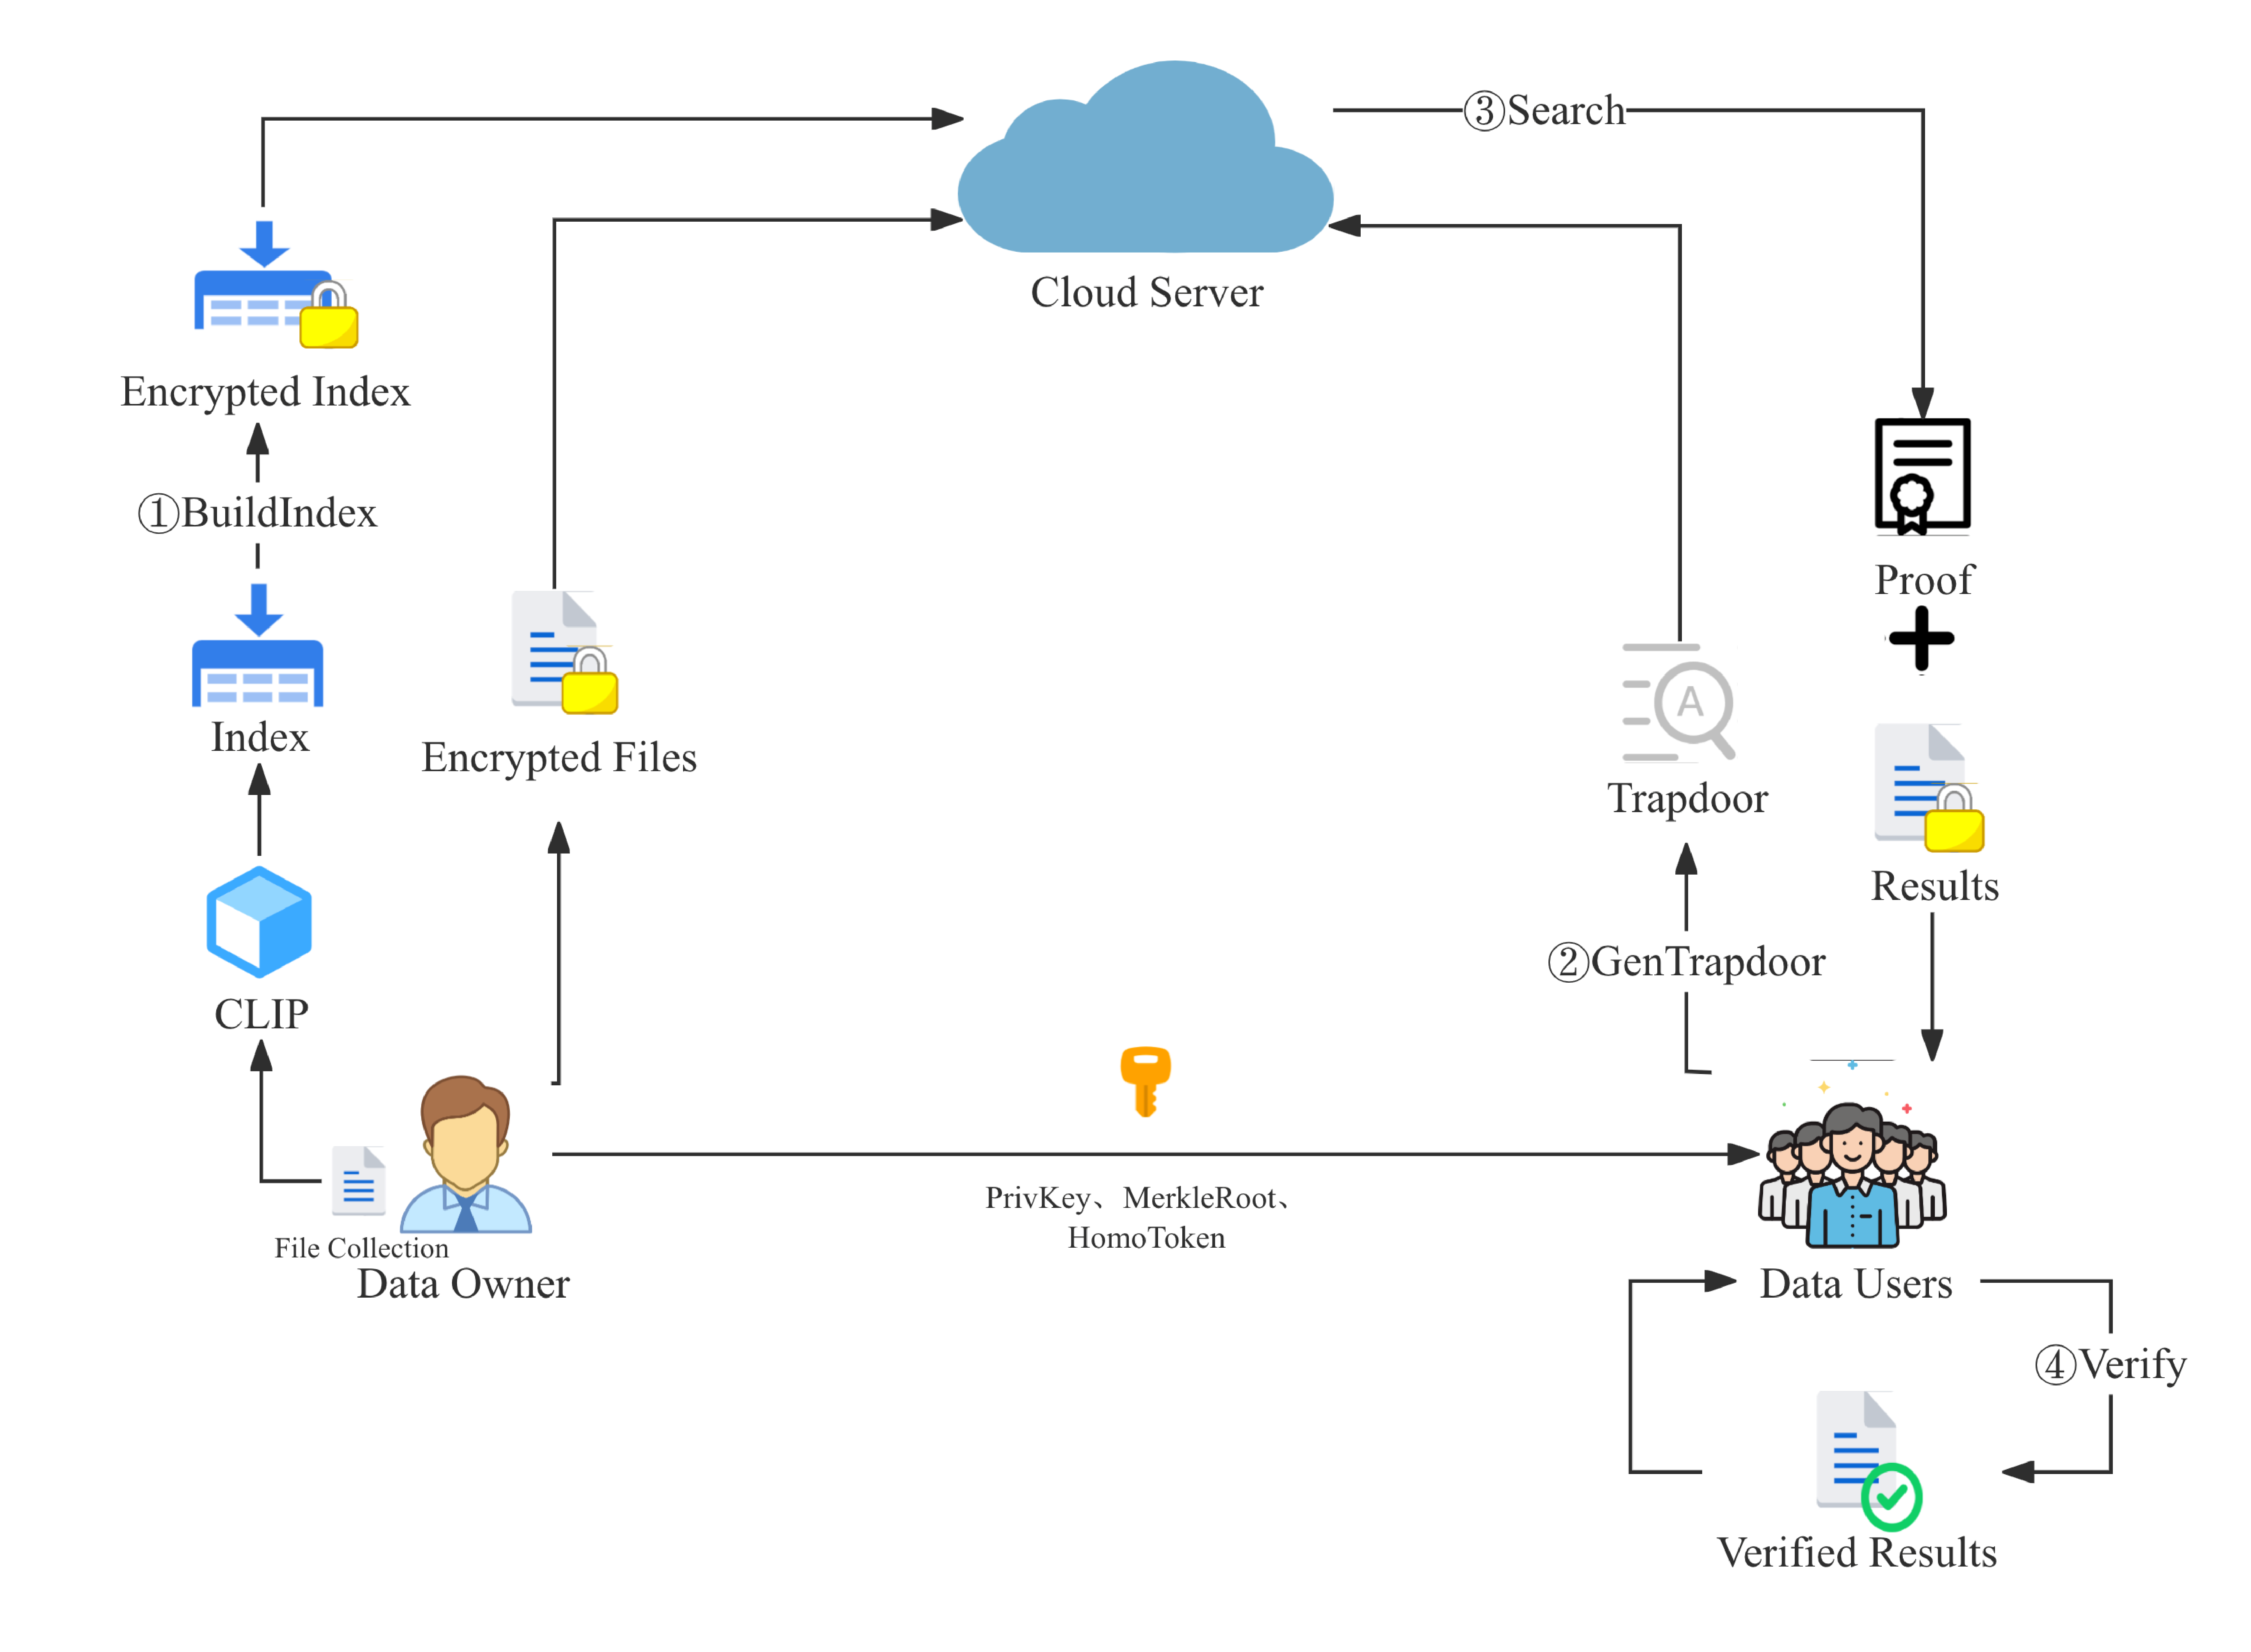
\includegraphics[width=0.48\textwidth]{figures/system_model.pdf}%
}{%
\IfFileExists{figures/system_model.png}{%
  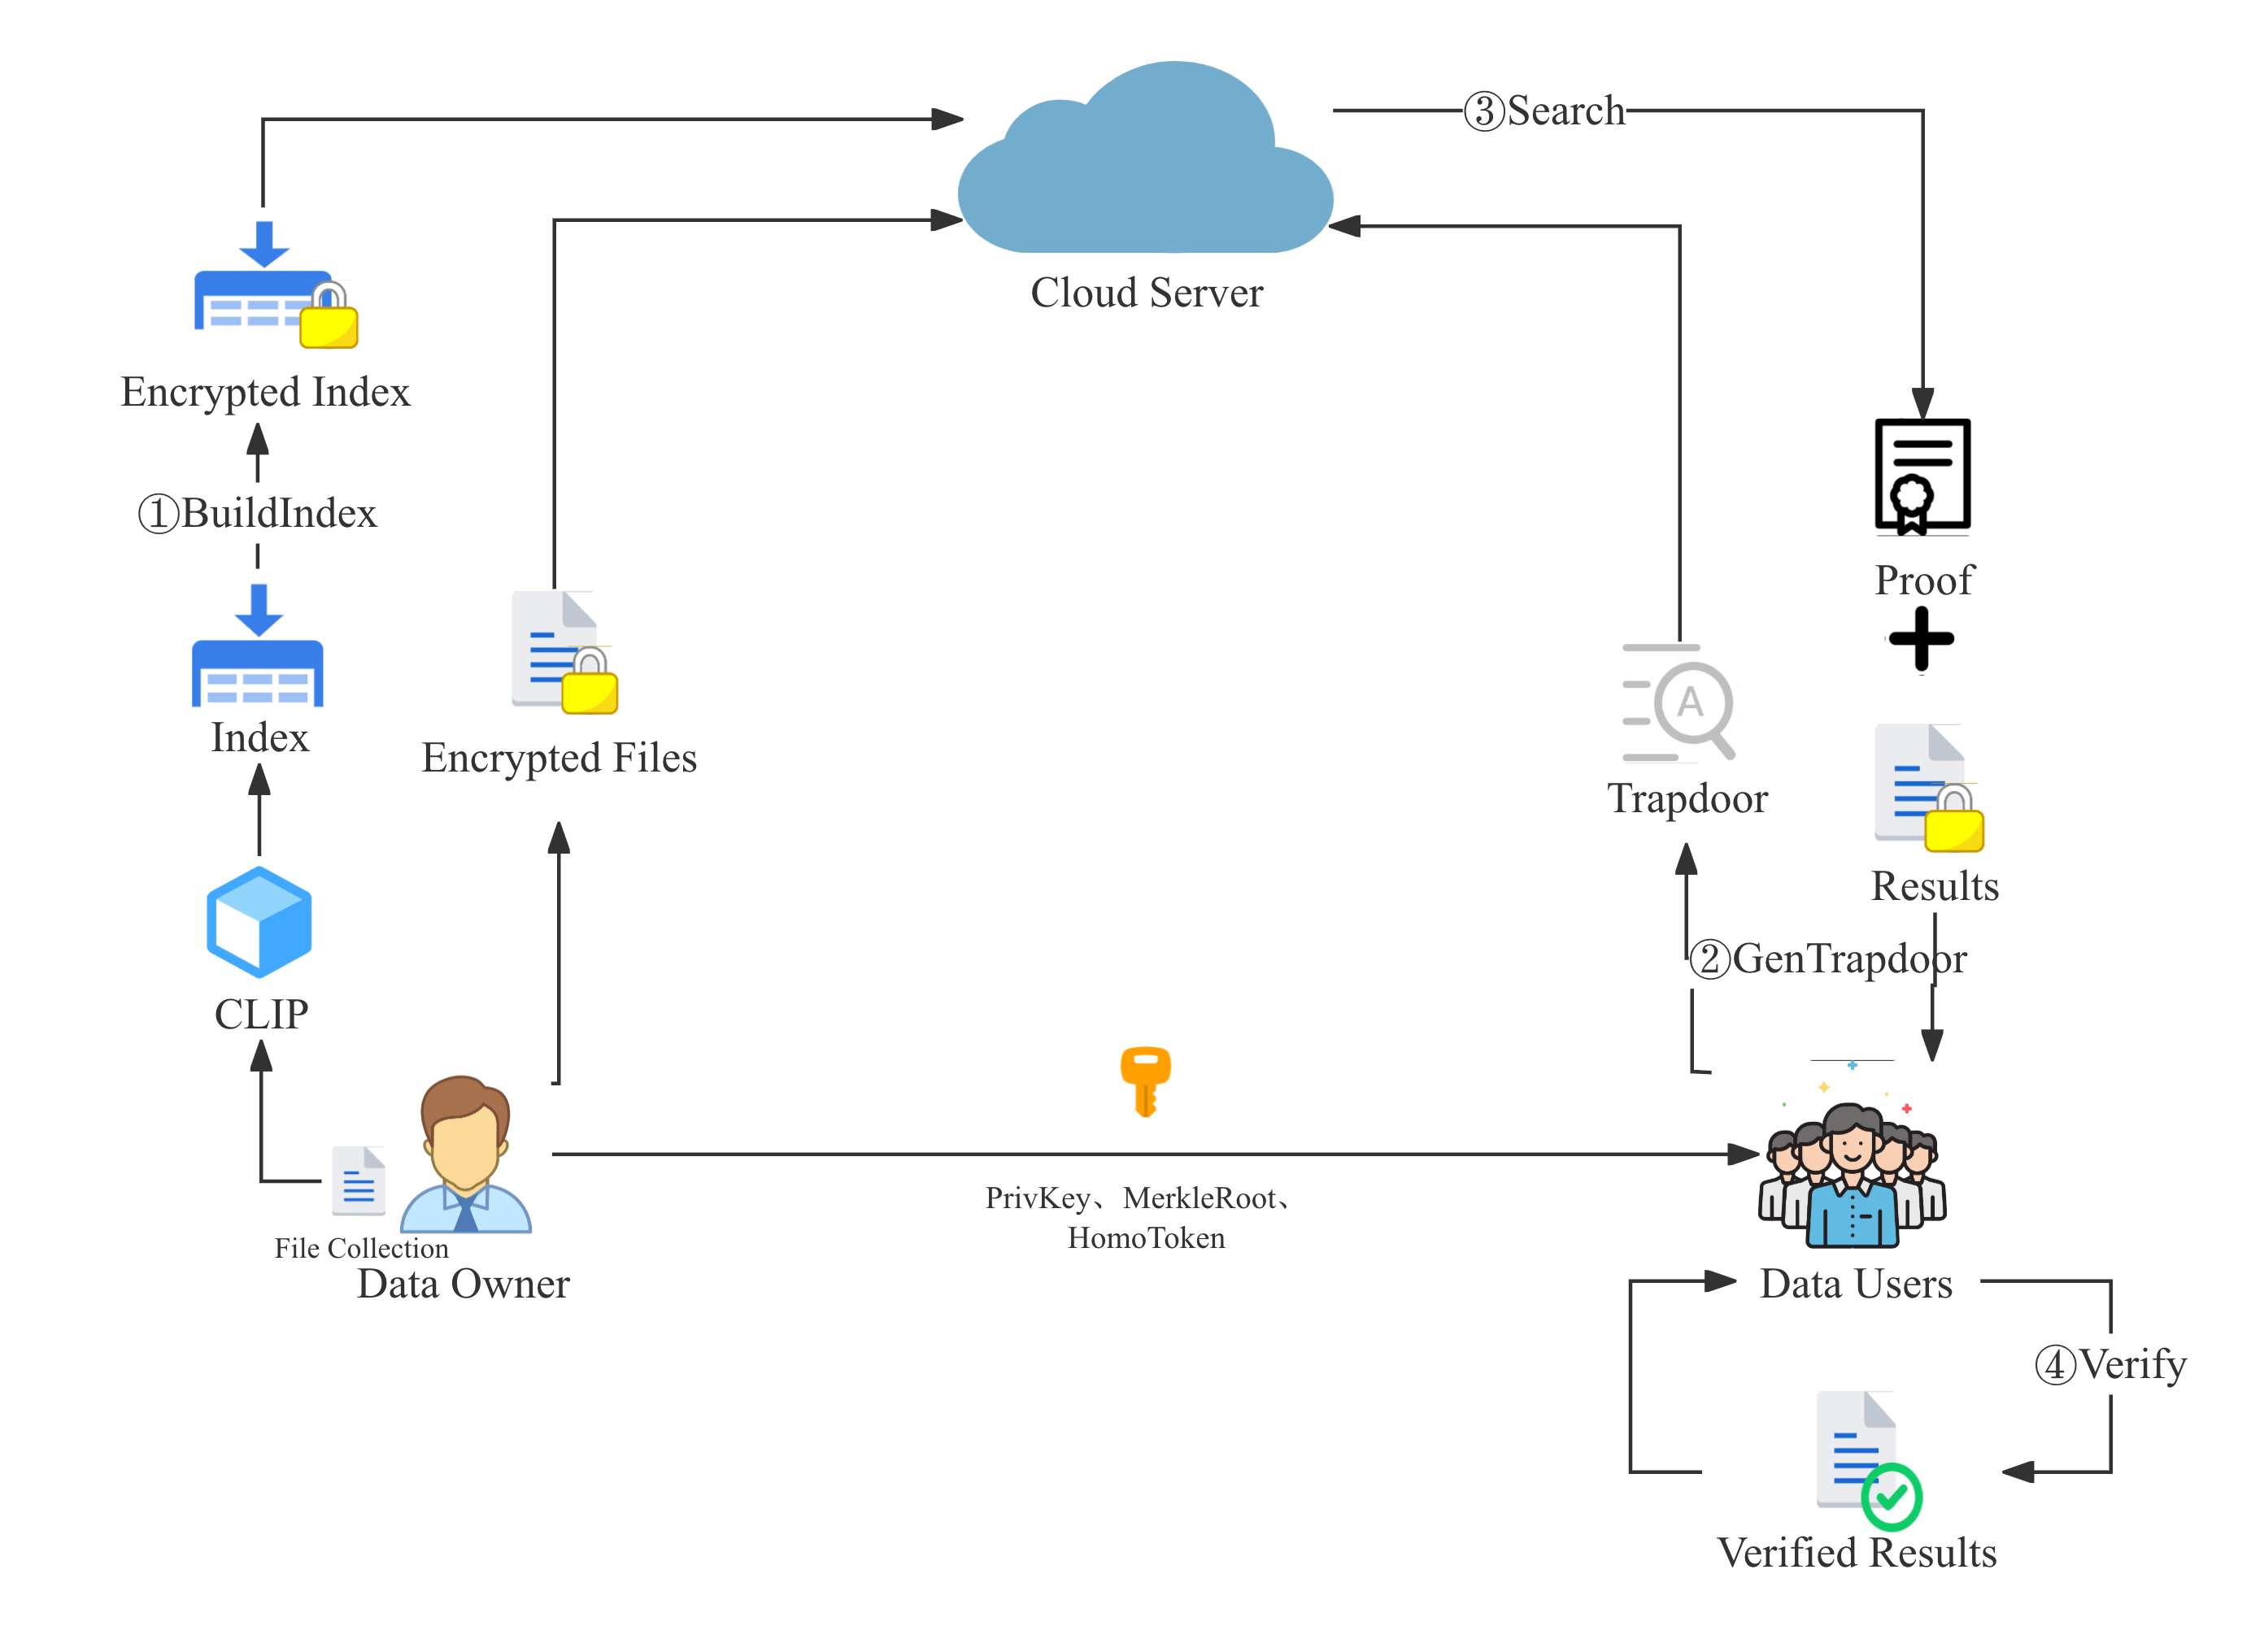
\includegraphics[width=0.48\textwidth]{figures/system_model.png}%
}{%
  \includesvg[width=0.48\textwidth]{figures/system_model}%
}}
\caption{System model of VCSE-HST. DO builds encrypted hierarchical spherical tree indexes and uploads to CS. DUs obtain keys from DO and submit encrypted queries to CS, which returns top-$k$ encrypted results. DUs verify the correctness of results.}
\label{fig:system}
\end{figure}

Before outsourcing data, the Data Owner (DO) extracts feature vectors from multimedia files using CLIP, normalizes them to the unit sphere, and builds a hierarchical $k$-ary spherical tree index using recursive $k$-means clustering. Each node in the tree stores an encrypted spherical center vector. DO then encrypts all tree nodes and data files before uploading them to the Cloud Server (CS) (\textcircled{1}BuildIndex). When a Data User (DU) wants to search, he/she first generates a trapdoor locally (\textcircled{2}GenTrapdoor), then submits the encrypted query trapdoor to CS (\textcircled{3}Search). CS performs beam search on the encrypted tree, computes similarity scores in the encrypted domain, and returns top-$k$ encrypted results to DU. Finally, DU verifies the correctness and completeness of the returned results (\textcircled{4}Verify).

\subsection{Problem Definition}

Let $\mathcal{F} = \{f_1, f_2, \ldots, f_n\}$ be a set of $n$ multimedia files. Using a pre-trained cross-modal model (e.g., CLIP), we extract a $d$-dimensional feature vector $\mathbf{v}_i \in \mathbb{R}^d$ for each file $f_i$. We normalize each vector to the unit sphere: $\mathbf{d}_i = \mathbf{v}_i / \|\mathbf{v}_i\|_2$, so that $\|\mathbf{d}_i\|_2 = 1$.

For a query $q$ (which can be text or image), we similarly extract and normalize its feature vector $\mathbf{q} \in \mathbb{R}^d$ with $\|\mathbf{q}\|_2 = 1$. The relevance score between a file $f_i$ and query $q$ is measured by the inner product (equivalently, cosine similarity for normalized vectors):

\begin{equation}
\mathcal{S}(\mathbf{d}_i, \mathbf{q}) = \mathbf{d}_i \cdot \mathbf{q} = \sum_{j=1}^{d} d_{i,j} \cdot q_j
\end{equation}

The goal of cross-modal searchable encryption is to find the top-$k$ files with the highest relevance scores over encrypted data, without revealing file content, query information, or relevance scores to CS.

\textbf{Efficiency Metric}: For $n$ files, the search complexity of linear search is $O(n)$. Tree-based methods aim to achieve sublinear complexity $O(\log n)$ or better through hierarchical pruning.

\textbf{Accuracy Metric}: We use Recall@K to measure accuracy:
\begin{equation}
\text{Recall@K} = \frac{\text{\# queries where top-K contains target class}}{{\text{\# total queries}}}
\end{equation}

In evaluation, we also report \textbf{Agree@1}, defined as the fraction of queries where the top-1 result returned by VCSE-HST matches the top-1 returned by the Cross-Model-SE baseline (used to quantify fidelity across beam sizes).

\subsection{Threat Model}

Following existing SSE schemes~\cite{miao2022ranked,yang2025secure}, we consider DO and DUs as fully trusted entities, while CS may be adversarial in two ways. Specifically:

\begin{itemize}
    \item \textbf{Adversarial CS}: CS may exhibit two types of adversarial behavior: (1) \emph{Confidentiality attacks} (honest-but-curious model): attempting to infer sensitive information from encrypted data, indexes, queries, and intermediate computation results; (2) \emph{Integrity attacks} (malicious model): reducing computational costs by executing incomplete searches (e.g., skipping expensive tree traversals, returning local optima, omitting required beam expansions, or forging result scores) while still reporting results to reduce operational overhead. CS has access to: (1) encrypted file vectors $\{\widehat{\mathbf{d}}_i\}$, (2) encrypted tree nodes $\{\widehat{\mathbf{c}}_j\}$, (3) encrypted query tokens $\widehat{\mathbf{q}}$, and (4) encrypted similarity scores $\mathcal{S}(\widehat{\mathbf{d}}_i, \widehat{\mathbf{q}})$. Our scheme addresses confidentiality via encryption and integrity via verifiable computation mechanisms.

    \item \textbf{Known Ciphertext Model}: CS only has access to encrypted data and encrypted queries, without additional background knowledge.

    \item \textbf{Known Background Model}: CS may have statistical information about the dataset (e.g., frequency distributions) and may attempt correlation attacks.
\end{itemize}

\textbf{Leakage scope}: Like most practical SSE schemes, we do not hide access patterns (which documents are returned) or search patterns (which tree nodes are visited during beam search). Protecting such patterns requires orthogonal techniques like ORAM~\cite{stefanov2018path} or distributed point functions~\cite{gilboa2014distributed} that incur substantial performance overhead; our focus is on achieving strong confidentiality and verifiable integrity within the standard leakage profile of tree-based SSE.

\section{Preliminaries}

\subsection{Bilinear Verification for Encrypted Inner Products}

In verifiable searchable encryption, two complementary mechanisms ensure result trustworthiness: \emph{correctness} (scores are computed accurately) and \emph{completeness} (all required operations are executed). We first introduce the bilinear verification technique that underpins our score correctness verification.

Let $\mathbf{E}\in\mathbb{R}^{2\ell}$ denote an encrypted document vector and $\mathbf{T}\in\mathbb{R}^{2\ell}$ a query trapdoor. The server reports an inner-product score $s=\langle \mathbf{T}, \mathbf{E}\rangle$. To enable verification without revealing plaintext, we augment the encryption with authentication vectors: for each document, a random secret tag $\mathbf{t}\in\mathbb{R}^{2\ell}$ and a secret verification parameter $\alpha>0$ (shared between DO and DUs via key distribution, unknown to CS) define an authentication vector $\mathbf{E}^{\mathsf{auth}}$ via
\begin{equation}
\alpha\,\mathbf{E}^{\mathsf{auth}} + \mathbf{E} = \mathbf{t}.
\end{equation}
Similarly, at query time, a random tag $\mathbf{r}\in\mathbb{R}^{2\ell}$ yields $\mathbf{T}^{\mathsf{auth}}$ satisfying
\begin{equation}
\alpha\,\mathbf{T}^{\mathsf{auth}} + \mathbf{T} = \mathbf{r}.
\end{equation}

The server computes $c_1=\langle \mathbf{T}, \mathbf{E}^{\mathsf{auth}}\rangle + \langle \mathbf{T}^{\mathsf{auth}}, \mathbf{E}\rangle$ and $c_2=\langle \mathbf{T}^{\mathsf{auth}}, \mathbf{E}^{\mathsf{auth}}\rangle$ without knowledge of $\mathbf{t}$ or $\mathbf{r}$, and returns $(s, c_1, c_2)$. The client then verifies the bilinear identity
\begin{equation}
\langle \mathbf{r}, \mathbf{t}\rangle = \alpha^2 c_2 + \alpha c_1 + s.
\end{equation}

This relation holds if and only if $s$ is the correct inner product; any tampering violates the identity with overwhelming probability (assuming the server does not know $\mathbf{t}$, $\mathbf{r}$, or $\alpha$). This mechanism guarantees \emph{score correctness} for returned items.

\subsection{Merkle Trees}

A Merkle tree~\cite{merkle1987digital} is a cryptographic commitment scheme for authenticated data structures. Given a rooted tree $\mathcal{T}$ and a collision-resistant hash function $H(\cdot)$, each node $u$ is assigned a hash value computed recursively:

\textbf{Standard Merkle Tree Construction.} For a leaf node $u$ storing data $\mathsf{data}(u)$:
\[
 H(u) = \mathsf{Hash}(\mathsf{data}(u)).
\]
For an internal node $u$ with children $v_1, v_2, \ldots, v_t$:
\[
 H(u) = \mathsf{Hash}(H(v_1) \| H(v_2) \| \cdots \| H(v_t)),
\]
where $\|$ denotes concatenation. The root hash $H(\textsf{root})$ serves as a compact commitment to the entire tree. To verify that a node $u$ is included in the tree, the prover provides a \emph{Merkle proof}: the sibling hashes along the path from $u$ to the root. The verifier recomputes hashes bottom-up and checks equality with the committed root $H(\textsf{root})$.

\textbf{Application to Our Hierarchical Index.} We apply Merkle trees to commit to our encrypted hierarchical spherical tree index. Each node $u$ carries metadata (encrypted center $\widehat{\mathbf{c}}_u$, node ID $\textsf{id}(u)$, and for leaves, document IDs $\mathsf{Docs}(u)$). We compute node hashes by incorporating this metadata:

For a leaf node $u$:
\[
 H(u)=\mathsf{Hash}(\textsf{id}(u)\,\|\,\widehat{\mathbf{c}}_u\,\|\,\mathsf{Docs}(u)\,\|\,\textsf{LEAF}).
\]
For an internal node $u$ with children $v_1,\ldots,v_t$:
\[
\begin{aligned}
 H(u) = \mathsf{Hash}(&\textsf{id}(u)\,\|\,\widehat{\mathbf{c}}_u\,\|\,\\
 &H(v_1)\,\|\,\cdots\,\|\,H(v_t)\,\|\,\textsf{INTERNAL}).
\end{aligned}
\]

The Data Owner publishes the Merkle root $H(\textsf{root})$. During search, the Cloud Server returns inclusion proofs for visited nodes. Under collision resistance, any tampering with the tree structure, node metadata, or search results will be detected with overwhelming probability.

\section{Proposed Scheme}
\label{sec:scheme}

In this section, we present the construction of VCSE-HST, including key generation, hierarchical spherical tree construction, index encryption, query token generation, beam search algorithm, and two complementary verification mechanisms. Our scheme provides \emph{score correctness verification} (ensuring returned similarity scores are computed accurately) via bilinear authentication vectors introduced in Preliminaries, and \emph{execution integrity verification} (ensuring the beam search algorithm is executed completely and correctly) via Merkle tree commitments. These two mechanisms work together to provide comprehensive verifiability: score correctness guarantees the mathematical accuracy of reported values, while execution integrity prevents the server from omitting required operations or fabricating non-existent results.

\subsection{Key Generation}

Given a security parameter $\kappa$, DO generates a secret key
\[
 SK=(\mathbf{s}, \mathbf{M}, \mathbf{M}^{-1}, \alpha, K_{\text{rule}}),
\]

where $\mathbf{s}\in\{0,1\}^{\ell}$ is a random splitting vector for the padded dimension $\ell$, $\mathbf{M}\in\mathbb{R}^{2\ell\times 2\ell}$ is a random invertible matrix (we use a symmetric construction in implementation), $\alpha>0$ is a secret verification parameter (kept from the server, shared only with authorized users), and $K_{\text{rule}}$ is an AES key used to encrypt the optional compression rule. This key setup follows an ASPE-style inner-product preserving transformation~\cite{wong2009secure}, which enables secure similarity computation over encrypted vectors while supporting efficient key management~\cite{liu2016efficient}.

\subsection{Hierarchical Spherical Tree Construction}

We propose a hierarchical $k$-ary spherical tree structure that achieves shallow depth and finer-grained semantic clustering.

\subsubsection{Spherical $k$-Means Clustering}

Given a set of normalized vectors $\{\mathbf{d}_1, \ldots, \mathbf{d}_m\}$ on the unit sphere, we use the following procedure.

\begin{algorithm}[t]
\caption{Spherical $k$-Means}
\label{alg:spherical_kmeans}
\begin{algorithmic}[1]
\REQUIRE Normalized vectors $\{\mathbf{d}_i\}_{i=1}^m$, branch factor $k$
\ENSURE Centers $\{\mathbf{c}_j\}_{j=1}^k$ and assignments
\STATE Initialize centers $\mathbf{c}_1,\ldots,\mathbf{c}_k$ by sampling from $\{\mathbf{d}_i\}$
\REPEAT
  \STATE Assignment: $\text{cluster}(i) \leftarrow \arg\max_j\; \mathbf{d}_i^{\top} \mathbf{c}_j$ for all $i$
  \STATE Update: $\mathbf{c}_j \leftarrow \frac{\sum_{i:\,\text{cluster}(i)=j} \mathbf{d}_i}{\big\|\sum_{i:\,\text{cluster}(i)=j} \mathbf{d}_i\big\|_2}$ for all $j$
\UNTIL convergence
\end{algorithmic}
\end{algorithm}

The key difference from Euclidean $k$-means is the normalization in updates so centers remain on the unit sphere.

\subsubsection{Recursive Tree Construction}

We build the hierarchical $k$-ary tree recursively as follows.

\begin{algorithm}[t]
\caption{Build Hierarchical Spherical Tree}
\label{alg:build_tree}
\begin{algorithmic}[1]
\REQUIRE Vectors $\{\mathbf{d}_1, \ldots, \mathbf{d}_m\}$, branch factor $k$, min cluster size $s_{\min}$, max depth $h_{\max}$
\ENSURE Root node of the hierarchical tree
\STATE Compute center $\mathbf{c} \leftarrow \frac{\sum_{i=1}^m \mathbf{d}_i}{\big\|\sum_{i=1}^{m} \mathbf{d}_i\big\|_2}$
\IF{$m \le s_{\min}$ or current depth $\ge h_{\max}$}
  \STATE Return a leaf node with center $\mathbf{c}$ and document IDs $\{1,\ldots,m\}$
\ELSE
  \STATE Run spherical $k$-means on $\{\mathbf{d}_i\}$ to obtain clusters $\{\mathcal{C}_1,\ldots,\mathcal{C}_k\}$
  \FOR{$j=1$ to $k$}
    \STATE Recursively build subtree $T_j$ on vectors in $\mathcal{C}_j$
  \ENDFOR
  \STATE Return an internal node with center $\mathbf{c}$ and children $\{T_1,\ldots,T_k\}$
\ENDIF
\end{algorithmic}
\end{algorithm}

On the full datasets, setting $k=10$ and $s_{\min}=20$ results in a tree with only 3--4 levels. Fig.~\ref{fig:tree_structure} provides a schematic view of the spherical-tree topology on the unit sphere: the hierarchical structure induces a nested partitioning where each internal node's center (L1) serves as a representative for its subtree, with child nodes (L2) forming local clusters in the vicinity of their parent on the sphere.

\begin{figure}[!t]
\centering
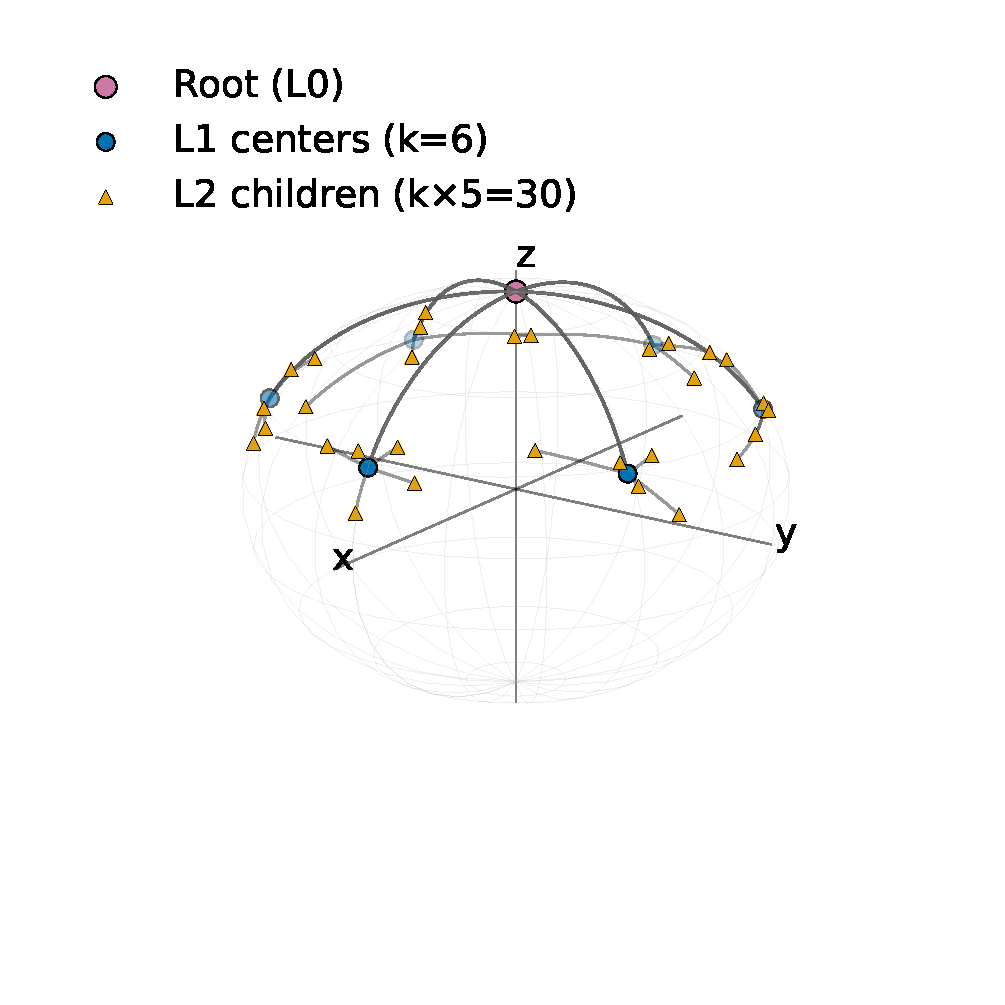
\includegraphics[width=0.48\textwidth]{figures/hierarchical_tree_structure.pdf}
\caption{Schematic hierarchical spherical tree on the unit sphere (illustrative example with $k{=}6$ branches shown for clarity). Blue markers indicate cluster centers (L1) and orange triangles show their child nodes (L2), connected via great-circle arcs. This spherical organization underlies our shallow $k$-ary index; in our experiments with $k{=}10$ on CIFAR-100, the tree depth is 3--4 layers.}
\label{fig:tree_structure}
\end{figure}


\subsection{Variance-Guided Dimension Reduction}
\label{subsec:variance_dr}

Our scheme incorporates a variance-guided dimension reduction module as a core preprocessing component. The module can be disabled by setting $k_\text{ratio}{=}0$ (yielding the no-compression baseline used in our main results), or enabled with configurable compression ratios to achieve memory/communication savings. Interestingly, our experiments reveal a non-monotonic recall pattern: modest compression (e.g., 0--10\% dimension removal) can sometimes \emph{improve} retrieval recall by eliminating low-variance dimensions that carry little discriminative power for the dataset, thereby reducing noise and enhancing cluster separation on the unit sphere. Sec.~\ref{sec:compression_study} reports detailed trade-offs across compression ratios.

\textbf{Rule generation.} Given the document embedding matrix $\mathbf{X}\in\mathbb{R}^{m\times n}$, we compute per-dimension variance $s_j=\mathrm{Var}(\mathbf{X}_{:,j})$ and select the $k$ smallest-variance dimensions to drop, where $k=\lfloor n\cdot k_\text{ratio}\rfloor$. Let $\mathcal{R}$ denote the set of indices to remove and $\mathcal{K}=[n]\setminus\mathcal{R}$ the kept indices.

\textbf{Encrypted rule.} The rule $\mathcal{R}$ is serialized and encrypted by AES-256-CBC using a key $K_\text{rule}$ generated during key setup. The ciphertext (with IV) is stored as part of the index metadata and is required at query time to ensure client/server consistency while hiding the exact rule.

\textbf{Document processing.} Each document vector is first restricted to $\mathcal{K}$, yielding a $d$-dimensional vector ($d=n-k$), then L2-normalized to the unit sphere before encryption.

\textbf{Query processing.} At query time, the client decrypts the encrypted rule and applies the same keep-set $\mathcal{K}$ to the query embedding, followed by L2-normalization and trapdoor generation. This guarantees that query and index share the same feature subspace without revealing the rule to the server.

This module is orthogonal to our hierarchical index and beam search. We report main results under $k_\text{ratio}=0$ (no compression) to focus on indexing/search; Sec.~\ref{sec:compression_study} (and Sec.~\ref{sec:compression_theory}) summarizes its impact succinctly.

\subsection{Index Encryption}

For each document $f_i$, DO first applies the optional compression rule (if enabled) to obtain a $d$-dimensional vector and L2-normalizes it. Then DO pads it to length $\ell$ by appending Gaussian noise in the last $\ell-d$ coordinates, yielding $\mathbf{v}_i\in\mathbb{R}^{\ell}$. We split $\mathbf{v}_i$ into two parts $\mathbf{v}_{i,1},\mathbf{v}_{i,2}\in\mathbb{R}^{\ell}$ according to $\mathbf{s}$:
\begin{equation}
\mathbf{v}_{i,1}[j],\,\mathbf{v}_{i,2}[j]=\begin{cases}
\mathbf{v}_i[j],\ \mathbf{v}_i[j], & \text{if } \mathbf{s}[j]=0,\\
r'_{i,j},\ \mathbf{v}_i[j]-r'_{i,j}, & \text{if } \mathbf{s}[j]=1,
\end{cases}
\end{equation}
where $r'_{i,j}$ are fresh random numbers. Concatenating $\mathbf{I}_i=[\mathbf{v}_{i,1};\mathbf{v}_{i,2}]\in\mathbb{R}^{2\ell}$ and multiplying by $\mathbf{M}^{\top}$ gives the encrypted index vector $\mathbf{E}_i=\mathbf{M}^{\top}\mathbf{I}_i$. For score-consistency verification, we also sample a random tag $\mathbf{t}_i\in\mathbb{R}^{2\ell}$ and publish $\mathbf{E}_i^{\mathsf{auth}}=(\mathbf{t}_i-\mathbf{E}_i)/\alpha$. Tree node centers are computed in plaintext (on normalized vectors), then encrypted in the same manner; we keep encrypted centers unnormalized in implementation.

Optionally, file contents $f_i$ can be encrypted as $f_i^*=\text{Enc}_{k_e}(f_i)$ using a symmetric cipher.

\subsection{Query Token Generation}

The client decrypts the AES-encrypted compression rule (if any) to obtain the keep-set, applies the same subspace to the query embedding, L2-normalizes it, and pads to $\ell$ with independent Gaussian noise, yielding $\mathbf{q}_{\text{pad}}\in\mathbb{R}^{\ell}$. Using the same splitting vector $\mathbf{s}$, we compute
\begin{equation}
\mathbf{q}_1[j],\,\mathbf{q}_2[j]=\begin{cases}
r_{q,j},\ \mathbf{q}_{\text{pad}}[j] - r_{q,j}, & \text{if } \mathbf{s}[j]=0,\\
\mathbf{q}_{\text{pad}}[j],\ \mathbf{q}_{\text{pad}}[j], & \text{if } \mathbf{s}[j]=1,
\end{cases}
\end{equation}
where $r_{q,j} \sim \mathcal{N}(0,1)$ are fresh random numbers sampled independently for each query and each coordinate. This randomized splitting (applied to coordinates where $\mathbf{s}[j]=0$) ensures that repeated queries produce computationally indistinguishable trapdoors, guaranteeing ciphertext indistinguishability and preventing correlation attacks. The splitting is complementary to index encryption: when $\mathbf{s}[j]=0$, the query splits randomly while the index keeps pairs equal; when $\mathbf{s}[j]=1$, the query keeps pairs equal while the index splits randomly. This duality preserves inner products. We then form $\mathbf{T}'=[\mathbf{q}_1;\mathbf{q}_2]$, and output the trapdoor $\mathbf{T}=\mathbf{M}^{-\top}\,\mathbf{T}'$. For verification, we also sample a random query tag $\mathbf{r}\in\mathbb{R}^{2\ell}$ and publish $\mathbf{T}^{\mathsf{auth}}=(\mathbf{r}-\mathbf{T})/\alpha$ alongside the query.

With these definitions, the encrypted inner-product score satisfies $\langle \mathbf{T}, \mathbf{E}_i\rangle = \langle \mathbf{T}', \mathbf{I}_i\rangle$, i.e., it equals the inner product in the padded subspace.

\subsection{Beam Search Algorithm}

Upon receiving the encrypted query token $\widehat{\mathbf{q}}$, CS performs beam search on the encrypted hierarchical tree $\widehat{\mathcal{T}}$ to find top-$k$ results. The key idea is to maintain $\beta$ candidate paths at each level instead of a single greedy path.

\begin{algorithm}[t]
\caption{Beam Search on Encrypted Hierarchical Tree}
\label{alg:beam_search}
\begin{algorithmic}[1]
\REQUIRE Encrypted tree $\widehat{\mathcal{T}}$, encrypted query $\widehat{\mathbf{q}}$, beam size $\beta$, top-$k$
\ENSURE Top-$k$ encrypted document IDs and scores
\STATE Initialize beam $\mathcal{B}_0 \leftarrow \{(\text{root},\, \mathcal{S}(\widehat{\mathbf{c}}_{\text{root}},\widehat{\mathbf{q}}))\}$, level $\ell\leftarrow 0$
\WHILE{$\mathcal{B}_\ell$ contains non-leaf nodes}
  \STATE Initialize next beam $\mathcal{B}_{\ell+1} \leftarrow \emptyset$
  \FOR{each node $u\in\mathcal{B}_\ell$}
    \IF{$u$ is a leaf}
      \STATE Add $u$ to $\mathcal{B}_{\ell+1}$
    \ELSE
      \FOR{each child $v$ of $u$}
        \STATE $s_v \leftarrow \mathcal{S}(\widehat{\mathbf{c}}_v, \widehat{\mathbf{q}})$; add $(v,s_v)$ to $\mathcal{B}_{\ell+1}$
      \ENDFOR
    \ENDIF
  \ENDFOR
  \STATE Prune $\mathcal{B}_{\ell+1}$ to top-$\beta$ nodes by score; $\ell\leftarrow \ell{+}1$
\ENDWHILE
\STATE Collect all document IDs from leaf nodes in $\mathcal{B}_\ell$
\STATE For each collected document $i$, compute exact score $s_i \leftarrow \mathcal{S}(\widehat{\mathbf{d}}_i, \widehat{\mathbf{q}})$
\STATE Return top-$k$ documents by $s_i$
\end{algorithmic}
\end{algorithm}

The encrypted similarity score is computed as the inner product $s_i=\langle \mathbf{T}, \mathbf{E}_i\rangle$. By construction of dual transforms, $\langle \mathbf{T}, \mathbf{E}_i\rangle=\langle \mathbf{T}', \mathbf{I}_i\rangle$, i.e., it equals the inner product in the padded subspace defined by the common rule, ensuring correctness under encryption.

%
% Removed beam search illustrative figure and description per request.
%
\textbf{Complexity Analysis}: For a tree with depth $h$ and branch factor $k$, beam search visits at most $O(\beta \cdot k \cdot h)$ nodes. With $h = \log_k n$, the complexity is $O(\beta k \log_k n)$. In practice with $k{=}10$ and modest $\beta$, the search visits only a small fraction of the corpus compared to linear scan.

\subsection{Merkle-Tree-Based Integrity Verification}
\label{subsec:merkle}

We augment VCSE-HST with a Merkle-tree-based integrity layer that enforces \emph{execution integrity} for beam search: (i) all required expansions are performed; (ii) global top-$\beta$ pruning is correct; and (iii) returned documents are included in the visited leaves. The design follows a two-layer commitment, aligned with our implementation and the detailed design in our documentation.

\begin{figure}[t]
\centering
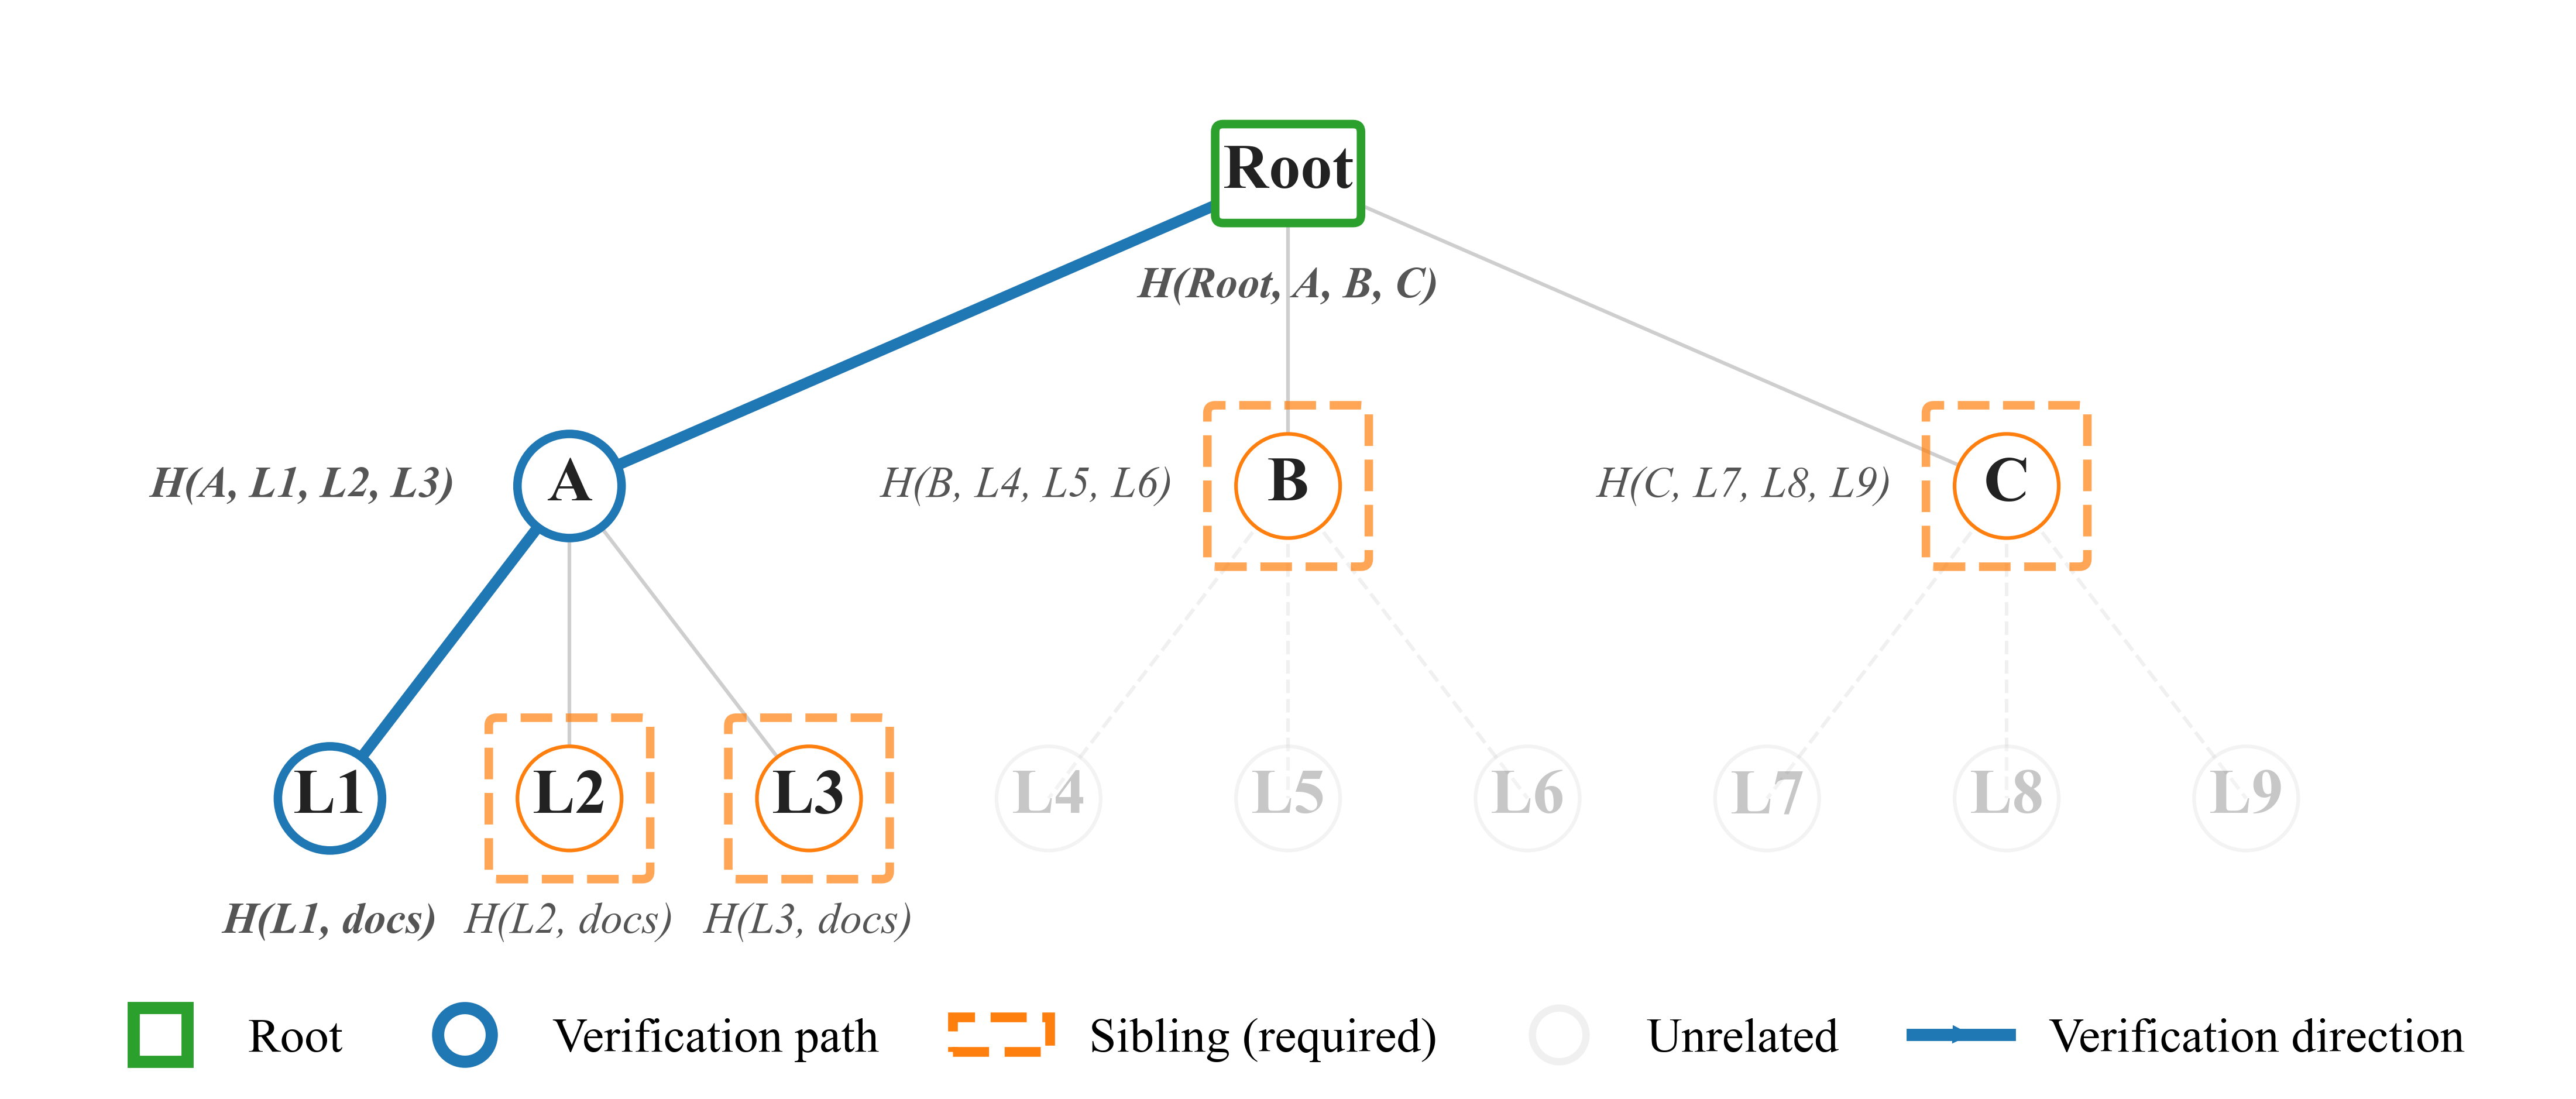
\includegraphics[width=\linewidth]{figures/merkle_beam_verification.png}
\caption{Merkle verification in a $k{=}3$ hierarchical tree with depth 2 (3 layers: root, internal nodes A/B/C, leaves L1--L9). To verify that leaf $L1$ is included in the committed tree, the server provides a verification path (blue nodes: $L1\rightarrow A\rightarrow \textsf{Root}$) and sibling hashes (orange dashed boxes: $\{L2, L3, B, C\}$). The client recomputes parent hashes bottom-up from $L1$ using the sibling values and checks that the recomputed root hash matches the published commitment $H(\textsf{Root})$. Hash formulas shown use simplified notation; full syntax with node IDs, metadata, and type tags is defined in Preliminaries.}
\label{fig:merkle_beam_verification}
\end{figure}

\textbf{Index commitment.} During index construction, DO computes a bottom-up Merkle tree over the hierarchical index. For each leaf node $u$ with encrypted center $\widehat{\mathbf{c}}_u$ and document IDs $\mathsf{Docs}(u)$, we set
\[
 H(u)=\mathsf{Hash}(\textsf{id}(u)\,\|\,\widehat{\mathbf{c}}_u\,\|\,\mathsf{Docs}(u)\,\|\,\textsf{LEAF}).
\]
For each internal node with children $v_1,\ldots,v_t$ we set
\[
\begin{aligned}
 H(u) = \mathsf{Hash}(&\textsf{id}(u)\,\|\,\widehat{\mathbf{c}}_u\,\|\, \\
 &H(v_1)\,\|\,\cdots\,\|\,H(v_t)\,\|\,\textsf{INTERNAL}).
\end{aligned}
\]
In our implementation we also concatenate the ordered list of child IDs to bind the structural ordering, which is compatible and strengthens the commitment.
DO publishes and pins the Merkle root $H(\textsf{root})$.

\textbf{Search proofs.} For each level $\ell$, the server returns a level-proof containing: current beam node IDs, for every non-leaf beam node, \emph{all} children with their scores and Merkle inclusion paths, and the claimed next-beam IDs (top-$\beta$ by score globally at that level). The client verifies: (1) inclusion of all nodes via Merkle paths w.r.t. $H(\textsf{root})$; (2) continuity of beams across levels; (3) correctness of all scores using the score-consistency tags; and (4) correctness of pruning by recomputing the global top-$\beta$ set from the supplied expansions. Finally, the client checks that every returned document lies in the leaves of the last-level beam (via leaf proofs) and that the reported top-$k$ matches the highest verified scores among those candidates.

This enforcement guarantees integrity of the \emph{executed} beam search (path completeness and result inclusion for the specified $\beta$), while leaving the algorithmic approximation of beam search itself unchanged.

\section{Security Analysis}
\label{sec:security}

In this section, we analyze the security of VCSE-HST. We first formalize our security model and definitions, then provide confidentiality arguments and verification mechanisms, and finally prove security theorems.

\subsection{Security Model and Definitions}

We formalize security using the standard leakage-based paradigm for searchable encryption. Let $\lambda$ denote the security parameter.

\textbf{Adversary model.} For \emph{confidentiality}, we consider an honest-but-curious server observing encrypted indexes and query trapdoors. For \emph{verifiability}, we allow a malicious server that can arbitrarily deviate from the protocol. Our scheme enforces score correctness (Theorem~\ref{thm:soundness}) and \emph{execution integrity} of beam search (path completeness and result inclusion for the chosen $\beta$) via Merkle commitments and level-by-level proofs.

\textbf{Leakage function.} We define $\mathcal{L}=(\mathcal{L}_{\mathrm{Index}},\mathcal{L}_{\mathrm{Search}})$:
\begin{align*}
\mathcal{L}_{\mathrm{Index}}(\mathcal{V}) &=\{m, d, \ell\}, \\
\mathcal{L}_{\mathrm{Search}}(q,\mathcal{V}) &=\{\mathrm{SP}(q),\,\mathrm{AP}(q,\mathcal{V})\}.
\end{align*}
where $m$ is the number of documents, $d$ is the feature dimension after optional compression, $\ell$ is the padded dimension, $\mathrm{SP}$ is the search pattern (repeated queries), and $\mathrm{AP}$ is the access pattern (returned document identifiers). These leakages align with Sec.~\ref{sec:scheme} and our discussion on pattern leakage; we do not protect access patterns in this work.

\textbf{Index semantic security.} Informally, encrypted indexes $\{\mathbf{E}_i\}$ are computationally indistinguishable from random vectors given only $\mathcal{L}_{\mathrm{Index}}$. Formally, for any PPT adversary $\mathcal{A}$ there exists a simulator $\mathcal{S}$ such that $\mathrm{View}^{\mathrm{Real}}\approx_c\mathrm{View}^{\mathrm{Ideal}}$ under $\mathcal{L}$.

\textbf{Trapdoor indistinguishability.} For distinct queries $q_0,q_1$, the distributions of their trapdoors are computationally indistinguishable given $\mathcal{L}_{\mathrm{Search}}$ (in particular, revealing only $\mathrm{SP}$ and $\mathrm{AP}$).

\textbf{Verification soundness (score correctness).} Against a malicious server, any non-algebraic modification of reported scores is detected with overwhelming probability (Theorem~\ref{thm:soundness}). In addition, Merkle commitments ensure execution integrity of beam search as formalized below.

\subsection{Confidentiality: Simulation-Based Argument}
\label{subsec:confidentiality}

We sketch a standard simulator proof under high-entropy padding and ASPE-style split-and-transform. Let $\mathbf{I}_i\in\mathbb{R}^{2\ell}$ denote the split-and-pad representation of document $i$, and $\mathbf{E}_i=\mathbf{M}^{\top}\mathbf{I}_i$ the encrypted index.

\textbf{Simulator.} Given $\mathcal{L}_{\mathrm{Index}}(\mathcal{V})=\{m,d,\ell\}$, sample $m$ independent random vectors in $\mathbb{R}^{2\ell}$ for $\{\mathbf{E}_i^{\mathrm{sim}}\}$ and independent random tags for authentication metadata; for each search, sample trapdoors consistent with $\mathcal{L}_{\mathrm{Search}}$ (reusing trapdoors only to reflect $\mathrm{SP}$) and program outputs to match $\mathrm{AP}$.

\textbf{Indistinguishability rationale.} (i) Gaussian padding of $\ell{-}d$ coordinates adds high entropy; (ii) the per-coordinate splitting masks introduce randomization in complementary dimensions—for indexes, when $\mathbf{s}[j]=1$; for trapdoors, when $\mathbf{s}[j]=0$—ensuring fresh randomness in every encrypted vector; (iii) the global invertible transform $\mathbf{M}$ scrambles coordinates, and under high-entropy inputs the outputs are computationally close to random; (iv) the encrypted compression rule (AES-256) hides the kept-dimension set. Hence $\mathrm{View}^{\mathrm{Real}}\approx_c\mathrm{View}^{\mathrm{Ideal}}$ under $\mathcal{L}$.

\subsection{Score Correctness Verification}

We adopt a lightweight mechanism that lets the client check the \emph{correctness of the reported inner-product scores} under encryption. Execution integrity of beam search (path completeness and result inclusion) is enforced separately by Merkle commitments (Sec.~\ref{subsec:merkle}); we do not claim global top-$k$ optimality beyond the chosen beam algorithm. Concretely, let $\mathbf{E}$ denote an encrypted document vector and $\mathbf{T}$ the query trapdoor. During index construction, we additionally create an authentication vector $\mathbf{E}^{\mathsf{auth}}$ per document via a random secret tag $\mathbf{t}$ and a public parameter $\alpha>0$; similarly, during trapdoor generation we create $\mathbf{T}^{\mathsf{auth}}$ using a query-side random tag $\mathbf{r}$:

\begin{equation}
\alpha\,\mathbf{E}^{\mathsf{auth}} + \mathbf{E} = \mathbf{t},\qquad \alpha\,\mathbf{T}^{\mathsf{auth}} + \mathbf{T} = \mathbf{r}.
\end{equation}

For each returned document, the server outputs the score and two auxiliary coefficients
\begin{equation}
 s=\langle \mathbf{T}, \mathbf{E}\rangle,\quad c_1=\langle \mathbf{T}, \mathbf{E}^{\mathsf{auth}}\rangle + \langle \mathbf{T}^{\mathsf{auth}}, \mathbf{E}\rangle,\quad c_2=\langle \mathbf{T}^{\mathsf{auth}}, \mathbf{E}^{\mathsf{auth}}\rangle.
\end{equation}

Given $(s,c_1,c_2)$ and the trapdoor-side values $(\mathbf{T},\mathbf{T}^{\mathsf{auth}},\alpha,\mathbf{r})$, the client retrieves the per-document tag $\mathbf{t}$ from local storage (securely distributed by DO during key distribution, never sent to CS) and checks the bilinear identity
\begin{equation}
 \langle \mathbf{r}, \mathbf{t}\rangle = \alpha^2 c_2 + \alpha c_1 + s.
\end{equation}
This identity detects any tampering of the inner-product score $s$ for the returned items. This mechanism provides score \emph{correctness}; execution integrity of the beam traversal and result inclusion is covered by Merkle proofs (Sec.~\ref{subsec:merkle}). We do not claim global optimality beyond the beam-search approximation.

\subsection{Index and Query Confidentiality}

\textbf{Theorem 1}: VCSE-HST guarantees index and query confidentiality in both known ciphertext model and known background model, assuming CS does not obtain the secret keys $(\mathbf{M}, \mathbf{s})$.

\textbf{Proof}: CS observes encrypted document vectors $\{\mathbf{E}_i=\mathbf{M}^{\top}\mathbf{I}_i\}$ and encrypted trapdoors $\{\mathbf{T}=\mathbf{M}^{-\top}\mathbf{T}'\}$. For the index, unknowns include the split-and-pad representations $\{\mathbf{I}_i\}$ (of size $2\ell$ per document, randomized by $\mathbf{s}$ and per-coordinate masks) and the global matrix $\mathbf{M}$ (with $4\ell^2$ degrees of freedom). The number of linear observations from $\{\mathbf{E}_i\}$ is insufficient to solve for both $\{\mathbf{I}_i\}$ and $\mathbf{M}$ jointly; the system is underdetermined. Similarly for queries, observing $\mathbf{T}=\mathbf{M}^{-\top}\mathbf{T}'$ without $\mathbf{M}$ and the rule does not reveal the plaintext query. Padding noise further obscures true feature values. Hence CS cannot recover plaintext vectors.

Furthermore, the dummy dimensions $\{\varepsilon_{i,j}\}$ following a normal distribution $\mathcal{N}(\mu, \sigma^2)$ add additional randomness that obscures the true feature values, preventing statistical attacks even in the known background model. Similar randomization techniques have been employed in data hiding~\cite{zhang2012separable} and secret sharing schemes~\cite{shamir1979share} to enhance security. \hfill $\square$

\subsection{Token Indistinguishability}

\textbf{Theorem 2}: VCSE-HST achieves query token indistinguishability for the same query request.

\textbf{Proof}: For two query tokens $\widehat{\mathbf{q}}'$ and $\widehat{\mathbf{q}}''$ generated from the same query $q$, the trapdoor generation process incorporates fresh randomness at two stages: (1) for coordinates where $\mathbf{s}[j]=0$, the splitting introduces per-coordinate random masks via fresh random numbers $r_{q,j} \sim \mathcal{N}(0,1)$, producing independent random pairs $(\mathbf{q}_1[j], \mathbf{q}_2[j]) = (r_{q,j}, \mathbf{q}_{\text{pad}}[j] - r_{q,j})$ that sum to the query value; (2) padding dimensions are filled with independent Gaussian noise samples. 

Since both tokens use independent random samples for splitting and padding, their distributions are computationally indistinguishable even for the same underlying query. The probability that two independently generated tokens coincide is negligible in the dimension of the random space. Formally, let $\epsilon$ denote the number of split dimensions; the collision probability is at most $\gamma^\epsilon$ where $\gamma \ll 1/2$, which is negligibly small for typical values (e.g., $\epsilon \geq d/2$). \hfill $\square$

\subsection{Score Correctness and Execution Integrity}

\textbf{Theorem 3} (Soundness; score correctness).\label{thm:soundness} Under random tags $(\mathbf{t},\mathbf{r})$ and secret $\alpha$, any modification of the reported score $s$ (or the associated coefficients $c_1,c_2$) for a returned document will, except with negligible probability, violate the identity $\langle \mathbf{r}, \mathbf{t}\rangle = \alpha^2 c_2 + \alpha c_1 + s$.

\textbf{Proof (Sketch)}: The tags and $\alpha$ define linear relations $\alpha\,\mathbf{E}^{\mathsf{auth}}+\mathbf{E}=\mathbf{t}$ and $\alpha\,\mathbf{T}^{\mathsf{auth}}+\mathbf{T}=\mathbf{r}$. Expanding $\langle \mathbf{r}, \mathbf{t}\rangle$ gives $\alpha^2\langle \mathbf{T}^{\mathsf{auth}},\mathbf{E}^{\mathsf{auth}}\rangle + \alpha(\langle \mathbf{T},\mathbf{E}^{\mathsf{auth}}\rangle + \langle \mathbf{T}^{\mathsf{auth}},\mathbf{E}\rangle) + \langle \mathbf{T},\mathbf{E}\rangle$, i.e., $\alpha^2 c_2 + \alpha c_1 + s$. Any change to $(s,c_1,c_2)$ that is not algebraically consistent will be detected with overwhelming probability against a server that does not know $(\alpha,\mathbf{t},\mathbf{r})$. This provides \emph{correctness} for reported scores; we do not claim global optimality beyond beam search. \hfill $\square$

\textbf{Theorem 4} (Execution integrity via Merkle commitments). Assume the hash function underlying the Merkle tree is collision resistant. Then any deviation by the server from the prescribed beam-search protocol at any level—(i) omitting children expansions for a beam node, (ii) injecting non-existent nodes, or (iii) misreporting the global top-$\beta$ pruning result—will be detected by the client with overwhelming probability using the level-by-level inclusion proofs and verified scores.

\textbf{Proof (Sketch).} For (ii), any injected node lacks a valid Merkle inclusion proof to the committed root, so verification fails by collision resistance. For (i), the client reconstructs, from the parent node’s inclusion proof, the expected set of child IDs; any missing child in the reported expansions is detected by set mismatch. For (iii), the client recomputes all verified children scores at the level (using score-consistency) and deterministically recomputes the global top-$\beta$ set; any discrepancy with the server’s claimed next beam is detected. The final result inclusion is verified by checking that all returned documents belong to the leaves reached by the last-level beam via leaf inclusion proofs. \hfill $\square$

\subsection{Privacy Leakage Discussion}

While VCSE-HST protects index, query, and keyword privacy, it does leak some information through the tree structure and search pattern:

\begin{itemize}
    \item \textbf{Tree structure leakage}: CS knows the hierarchical structure of the tree (which documents are in the same subtree), but not the semantic meaning of clusters due to encrypted node centers.
    
    \item \textbf{Search pattern leakage}: CS observes which tree nodes are visited during beam search, revealing information about the query's similarity pattern. Beam search visits multiple paths and thus leaks the set of explored nodes; we do not claim any privacy benefit over greedy search.
    
    \item \textbf{Access pattern leakage}: CS knows which documents are returned for each query. This is common in most SSE schemes and can be mitigated using ORAM techniques if needed.
\end{itemize}

The security-privacy trade-off can be adjusted by tuning the noise parameter $\sigma$ in dummy dimensions and the beam size $\beta$. Larger $\sigma$ provides stronger privacy but may reduce accuracy, while larger $\beta$ visits more tree nodes but provides more search diversity.
\section{Performance Evaluation}
\label{sec:evaluation}

In this section, we present extensive experiments to evaluate the performance of VCSE-HST, comparing it with state-of-the-art methods including Cross-Model-SE~\cite{yang2025secure} and linear search baseline.

\subsection{Experimental Setup}
\textbf{Dataset}: We evaluate on two large-scale datasets. (i) \textbf{CIFAR-100}~\cite{krizhevsky2009learning}: we use the full training split with 50{,}000 images and 100 text queries (one per class). (ii) \textbf{Caltech256}: we use the full dataset with 30{,}607 images and 257 text queries (one per class).

\textbf{Feature Extraction}: We use the pre-trained CLIP model (ViT-B/32)~\cite{radford2021learning} to extract 512-dimensional features for both images and text queries. All features are normalized to the unit sphere.

% TODO: 【实验平台信息不足】虽然提到了M1处理器，但缺少关键信息：
% 1. M1芯片的具体型号（M1/M1 Pro/M1 Max/M1 Ultra）
% 2. 操作系统版本（macOS版本）
% 3. Python和NumPy的具体版本
% 4. 是否使用了硬件加速（如Metal/Accelerate框架）
% 5. 实验是否在多个机器上重复以验证可重复性
% 另外，M1的性能与标准x86服务器差异较大，这可能影响与其他论文的性能对比的公平性。
\textbf{Implementation}: The experiments are conducted on a machine with Apple Silicon M1 processor and 16GB RAM. We implement VCSE-HST in Python 3.10 using NumPy for matrix operations.

\textbf{Parameters}:
\begin{itemize}
    \item Tree construction: branch factor $k=10$, min cluster size $s_{\min}=20$
    \item Encryption: no dimension compression ($k_{\text{ratio}}=0$); padding ratio $\ell/d \in \{1.0, 1.05\}$; noise on padding $\sigma = \sigma_q \in \{0.0, 0.01\}$
    \item Beam search: beam size $\beta \in \{1, 3, 7, 10\}$
    \item Top-$k$ results: $k \in \{1, 5, 10\}$
\end{itemize}

\textbf{Evaluation Metrics}:
\begin{itemize}
    \item \textbf{Recall@K}: Fraction of queries where the top-$K$ results contain at least one document from the target class
    \item \textbf{Agree@1}: Fraction of queries where the top-1 result returned by VCSE-HST matches the top-1 returned by the Cross-Model-SE baseline (fidelity to baseline)
    \item \textbf{Search Time}: Average time per query (ms)
    \item \textbf{Speedup}: Ratio of baseline search time to our method's search time
\end{itemize}

\textbf{Baselines}:
\begin{itemize}
    \item \textbf{Linear Search}: Exhaustive search over all encrypted documents
    \item \textbf{Cross-Model-SE}: LSH-based cross-modal searchable encryption~\cite{yang2025secure} with 64 hash tables and hash dimension 128
\end{itemize}

\vspace{2pt}

\subsection{Overall Performance Comparison}

Tables~\ref{tab:comparison_cifar_full} and~\ref{tab:comparison_caltech_full} summarize performance on the full CIFAR-100 (50{,}000 images) and Caltech256 (30{,}607 images) datasets. Note that the recall rates reflect the CLIP model's retrieval capability, not limitations of the encryption schemes. Thus, accuracy metrics are only compared among CLIP-based schemes (Cross-Model-SE, Linear Search, and VCSE-HST). Cross-Model-SE with tuned parameters (64 tables, 128-dim hashes) reaches 90\% R@1 on CIFAR-100 and serves as the latency baseline (\~57.5ms/query). VCSE-HST with beam size 10 matches 90\% R@1 while being 7.5$\times$ faster (\~7.66ms/query); with beam size 3, it yields up to 19.7$\times$ speedup (\~2.91ms/query) with only \~7\% R@1 loss. On Caltech256, beam size 10 similarly achieves \~7.5$\times$ speedup at comparable accuracy.

We also compare with MU-TEIR~\cite{yang2022mu} and PITR~\cite{zhang2024efficient} in terms of computational overhead. Since these schemes use different feature extraction models, only time and memory metrics are compared (accuracy comparison would be meaningless). Detailed performance metrics are shown in Table~\ref{tab:comparison_cifar_full}. The optional compression module is evaluated separately in Sec.~\ref{sec:compression_study}.

\begin{table*}[!t]
\centering
\caption{Performance comparison on CIFAR-100 (50{,}000 images, 100 queries)}
\label{tab:comparison_cifar_full}
\begin{tabular}{lccccccc}
\toprule
\textbf{Scheme} & \textbf{R@1} & \textbf{R@5} & \textbf{R@10} & \textbf{Agree@1} & \textbf{Search Time} & \textbf{Speedup}$^\dagger$ & \textbf{Index Size} \\
 & (\%) & (\%) & (\%) & (\%) & (ms) & (vs. Cross-Model-SE) & (MB) \\
\midrule
Cross-Model-SE & 90 & 97 & 98 & 100 & 57.47 & 1.0$\times$ & 518.89 \\
Linear Search & 90 & 97 & 98 & 100 & 144.44 & 0.4$\times$ & 782.10 \\
\midrule
VCSE-HST ($\beta=3$) & 83 & 96 & 97 & 70 & 2.91 & \textbf{19.7$\times$} & 782.10 \\
VCSE-HST ($\beta=7$) & 89 & 97 & 98 & 86 & 6.39 & \textbf{9.0$\times$} & 782.10 \\
VCSE-HST ($\beta=10$) & \textbf{90} & 97 & 99 & 90 & 7.66 & \textbf{7.5$\times$} & 782.10 \\
\midrule
MU-TEIR$^*$ & --- & --- & --- & --- & 12{,}570 & 0.005$\times$ & $\sim$60 \\
PITR$^*$ & --- & --- & --- & --- & 64 & 0.90$\times$ & 28.5 \\
\bottomrule
\multicolumn{8}{l}{\footnotesize $^\dagger$Speedup is calculated relative to Cross-Model-SE (avg. per-query time).} \\
\multicolumn{8}{l}{\footnotesize $^*$Accuracy metrics not comparable due to different feature extraction models.} \\
\end{tabular}
\end{table*}

\begin{table*}[!t]
\centering
\caption{Performance on Caltech256 (full: 30{,}607 images, 257 queries)}
\label{tab:comparison_caltech_full}
\begin{tabular}{lccccccc}
\toprule
\textbf{Scheme} & \textbf{R@1} & \textbf{R@5} & \textbf{R@10} & \textbf{Agree@1} & \textbf{Search Time} & \textbf{Speedup}$^\dagger$ & \textbf{Index Size} \\
 & (\%) & (\%) & (\%) & (\%) & (ms) & (vs. Cross-Model-SE) & (MB) \\
\midrule
Cross-Model-SE & 88.7 & 96.5 & 98.1 & 100 & 34.38 & 1.0$\times$ & 317.79 \\
Linear Search & 88.7 & 96.5 & 98.1 & 100 & 86.12 & 0.4$\times$ & 478.70 \\
\midrule
VCSE-HST ($\beta=10$) & \textbf{88.7} & 96.5 & 98.1 & 90 & 4.58 & \textbf{7.5$\times$} & 478.70 \\
\bottomrule
\multicolumn{8}{l}{\footnotesize $^\dagger$Speedup is calculated relative to Cross-Model-SE (avg. per-query time).} \\
\end{tabular}
\end{table*}

\textbf{Key Observations}:
\begin{enumerate}
    \item \textbf{Beam size provides flexible trade-offs}: By adjusting $\beta$ from 1 to 10, we can smoothly trade accuracy for speed. Beam size 3 offers the best cost-performance ratio (83\% R@1, 19.7$\times$ speedup), while beam size 10 achieves state-of-the-art accuracy with significant speedup.
    
    \item \textbf{Shallow tree structure is crucial}: Our 3--4 level hierarchical tree enables both fast search and high accuracy, avoiding the accumulated errors of deeper trees.
    
    \item \textbf{Superior to LSH-based methods}: VCSE-HST with beam size 10 matches Cross-Model-SE's 90\% Recall@1 while being 7.5$\times$ faster, demonstrating the effectiveness of hierarchical tree indexing combined with beam search.
\end{enumerate}

Fig.~\ref{fig:accuracy_comparison} visualizes the accuracy comparison across different recall metrics.

\begin{figure}[!t]
\centering
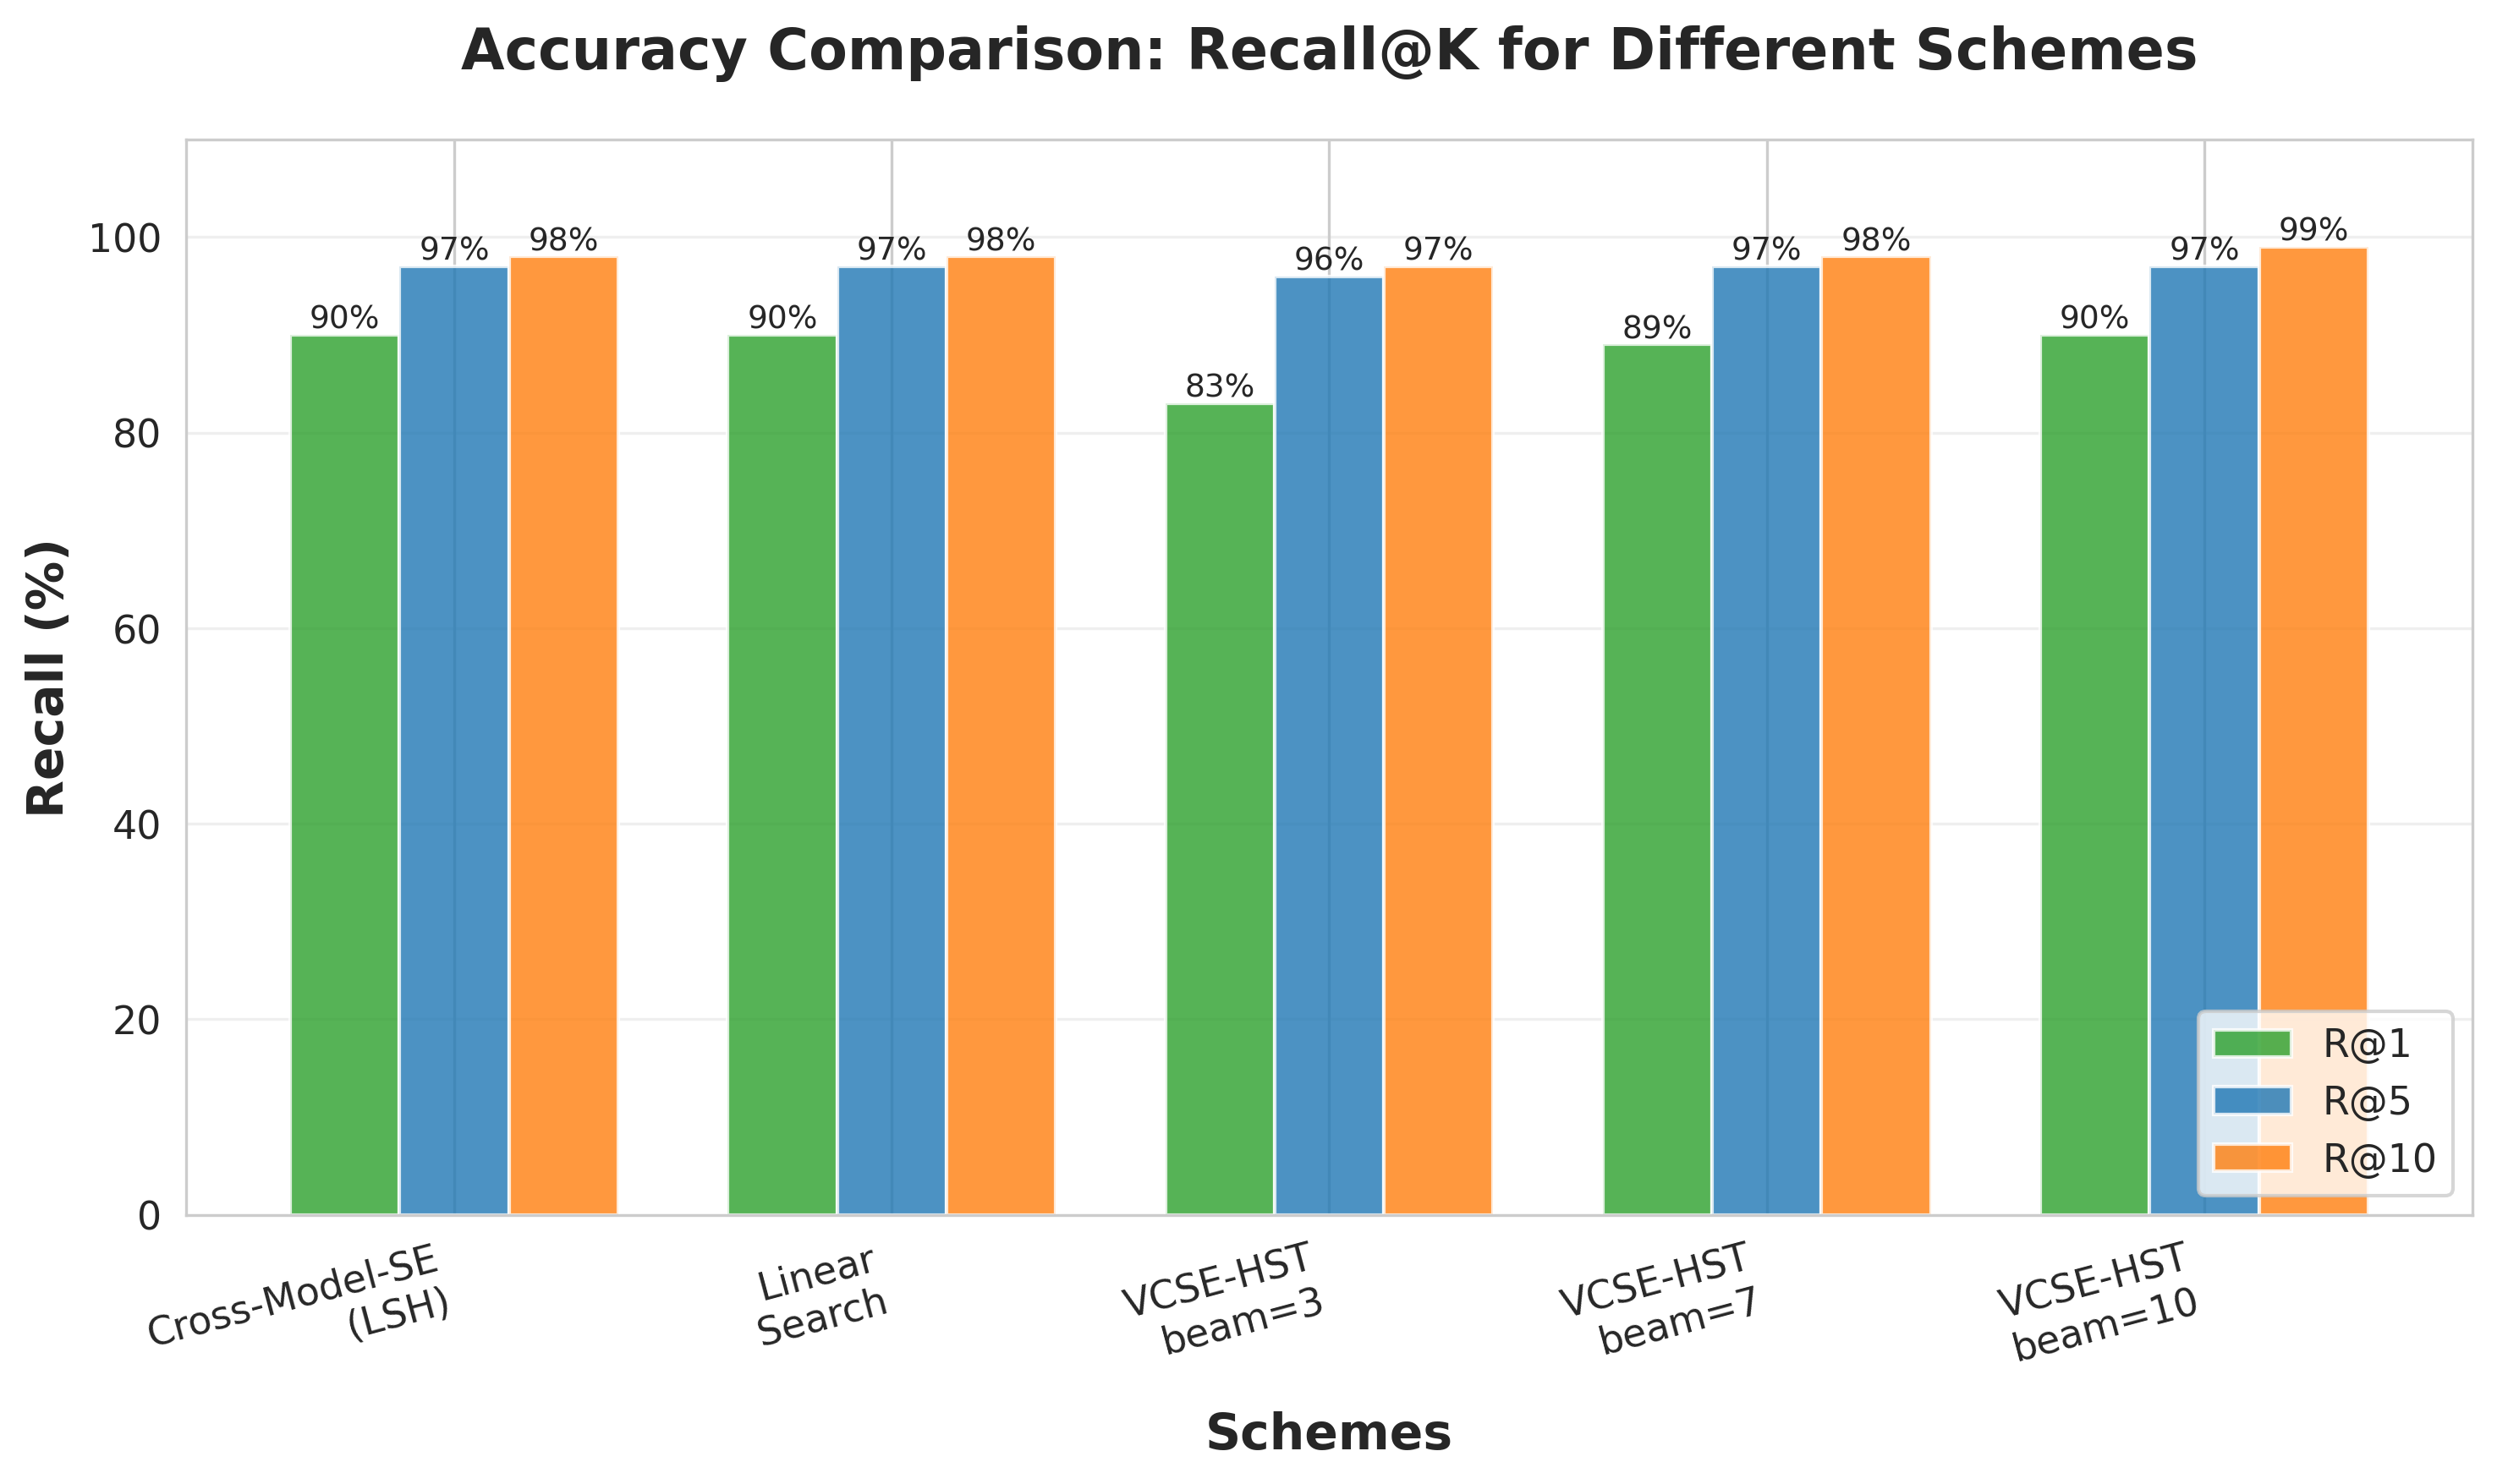
\includegraphics[width=0.48\textwidth]{figures/paper_accuracy_comparison.png}
\caption{Accuracy comparison (Recall@1, Recall@5, Recall@10) for different schemes. VCSE-HST with beam size 10 matches Cross-Model-SE's accuracy while being much faster. Even beam size 3 achieves competitive Recall@5 and Recall@10.}
\label{fig:accuracy_comparison}
\end{figure}

\subsection{Search Time Analysis}

Fig.~\ref{fig:search_time} compares average search time on a log scale; VCSE-HST attains 7.5--19.7$\times$ speedups over Cross-Model-SE under our settings.

\begin{figure}[!t]
\centering
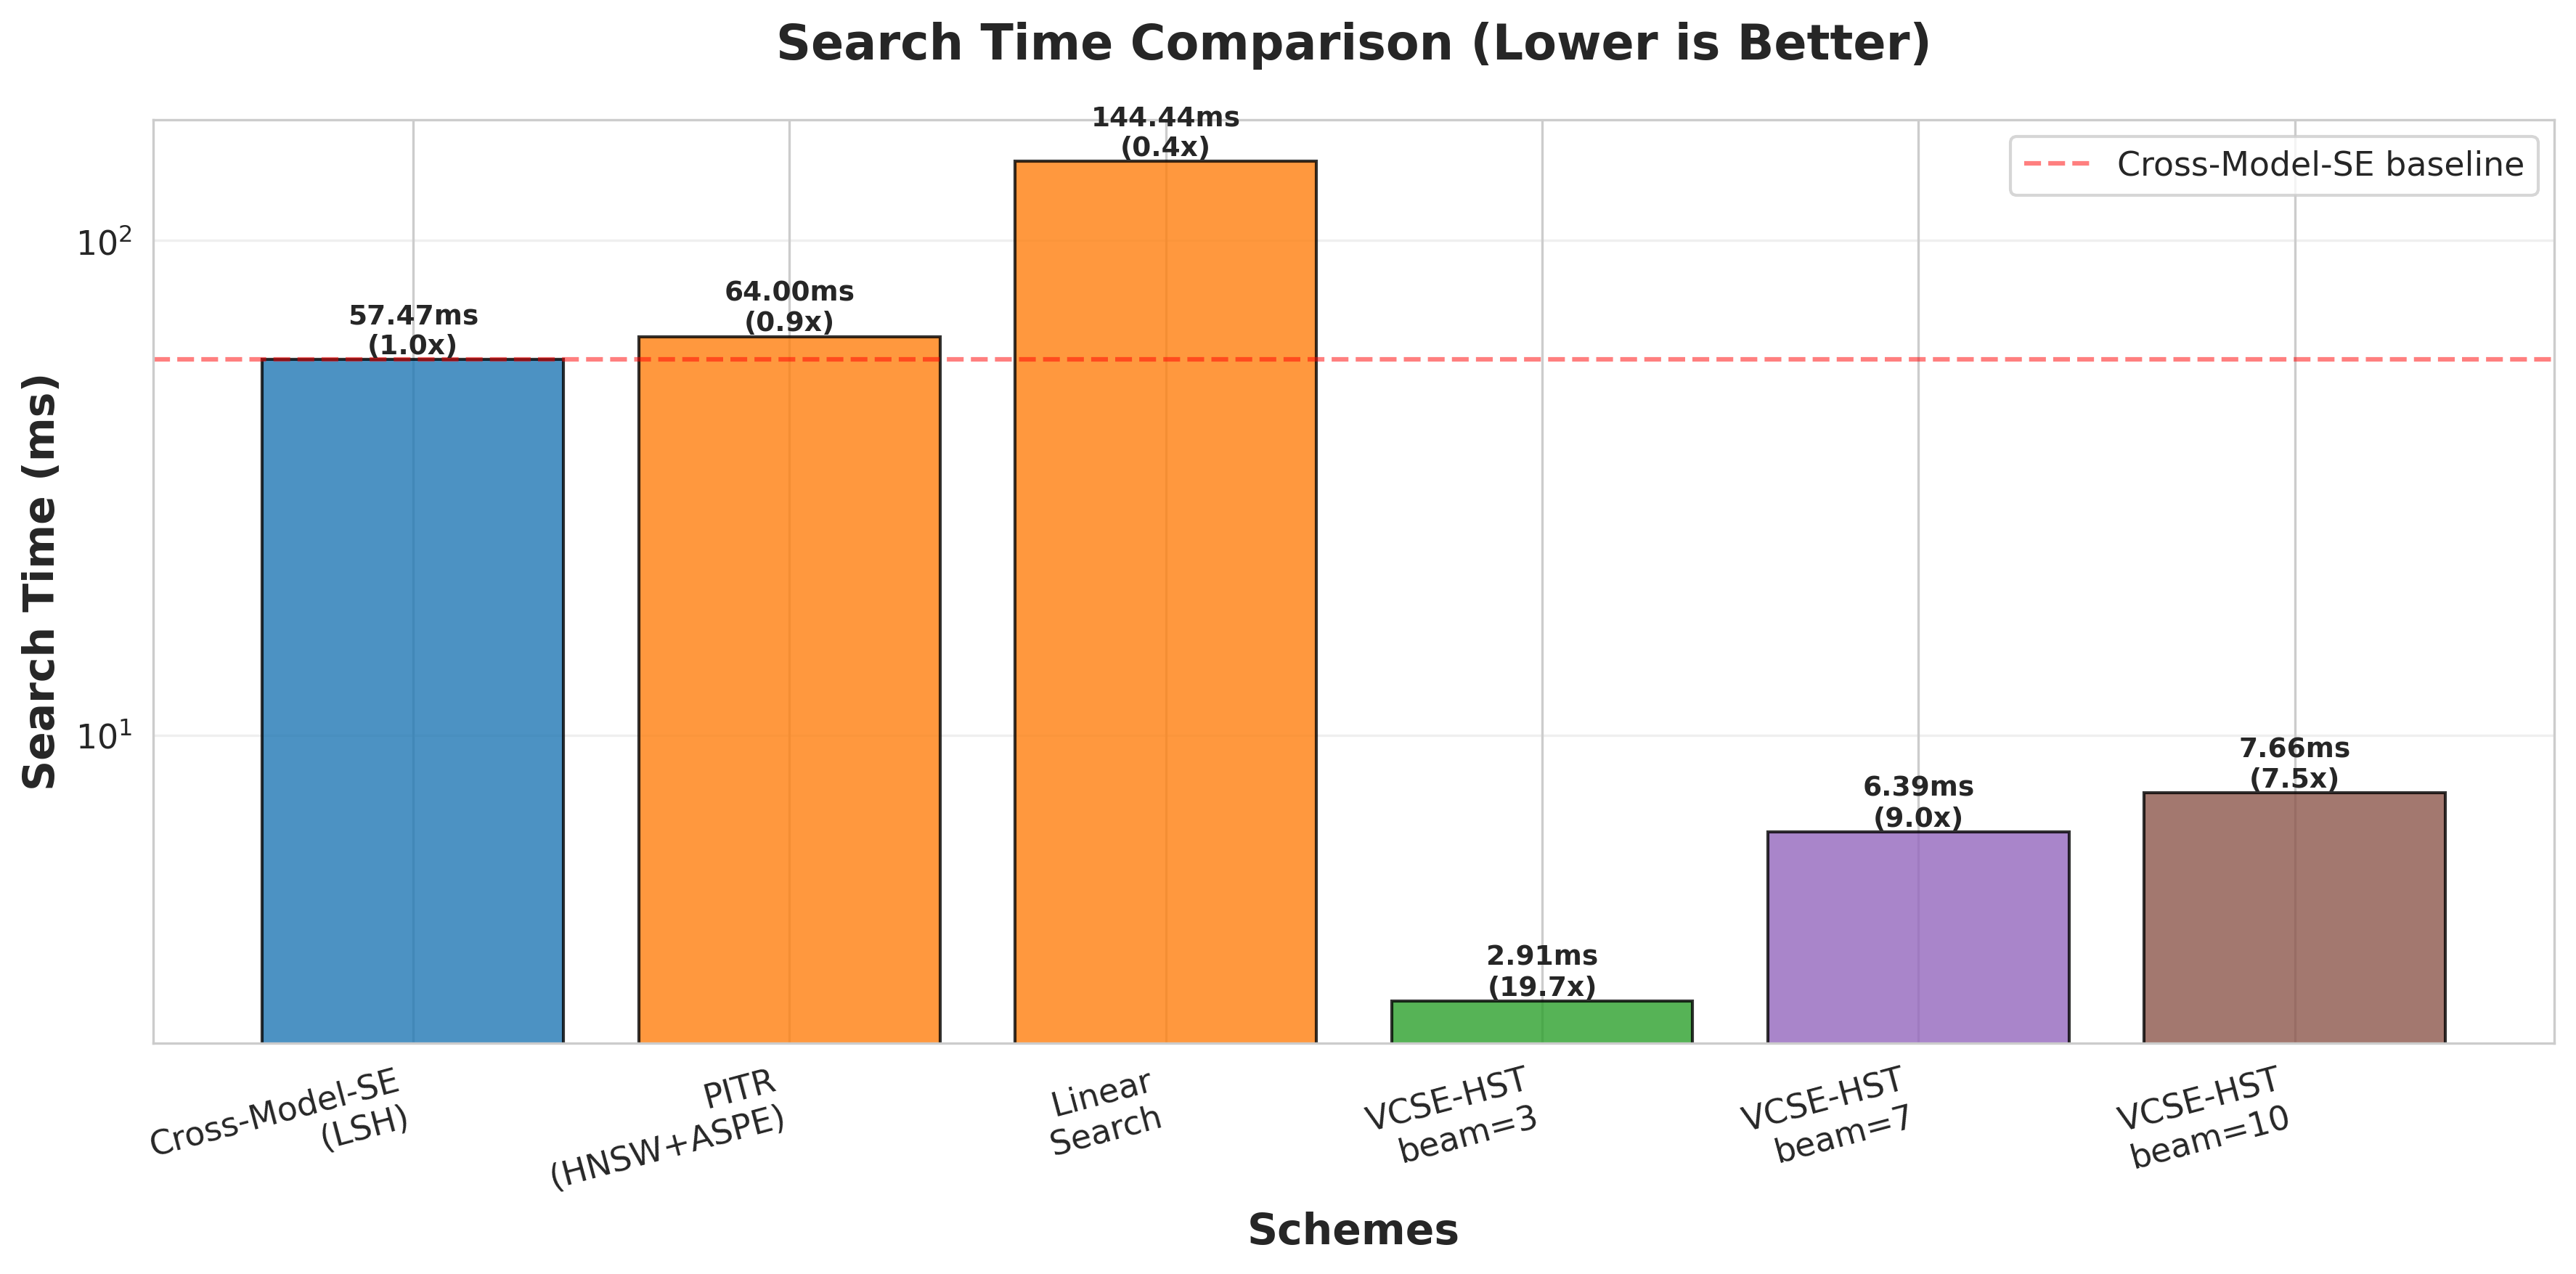
\includegraphics[width=0.48\textwidth]{figures/paper_search_time_comparison.png}
\caption{Search time comparison on logarithmic scale. VCSE-HST attains 7.5--19.7$\times$ speedup over Cross-Model-SE under our settings. Beam size 10 achieves single-digit millisecond latency.}
\label{fig:search_time}
\end{figure}

The millisecond-level search time of VCSE-HST is attributed to: (1) a shallow tree structure (3--4 levels), (2) efficient beam pruning that visits only a small fraction of nodes, and (3) optimized inner product computations on normalized vectors.
\subsection{Beam Size Trade-off Analysis}

We report accuracy and search time as beam size $\beta$ varies (no compression, no noise). Fig.~\ref{fig:beam_acc} and Fig.~\ref{fig:beam_time} present the two perspectives separately for clearer layout.

\begin{figure}[!t]
\centering
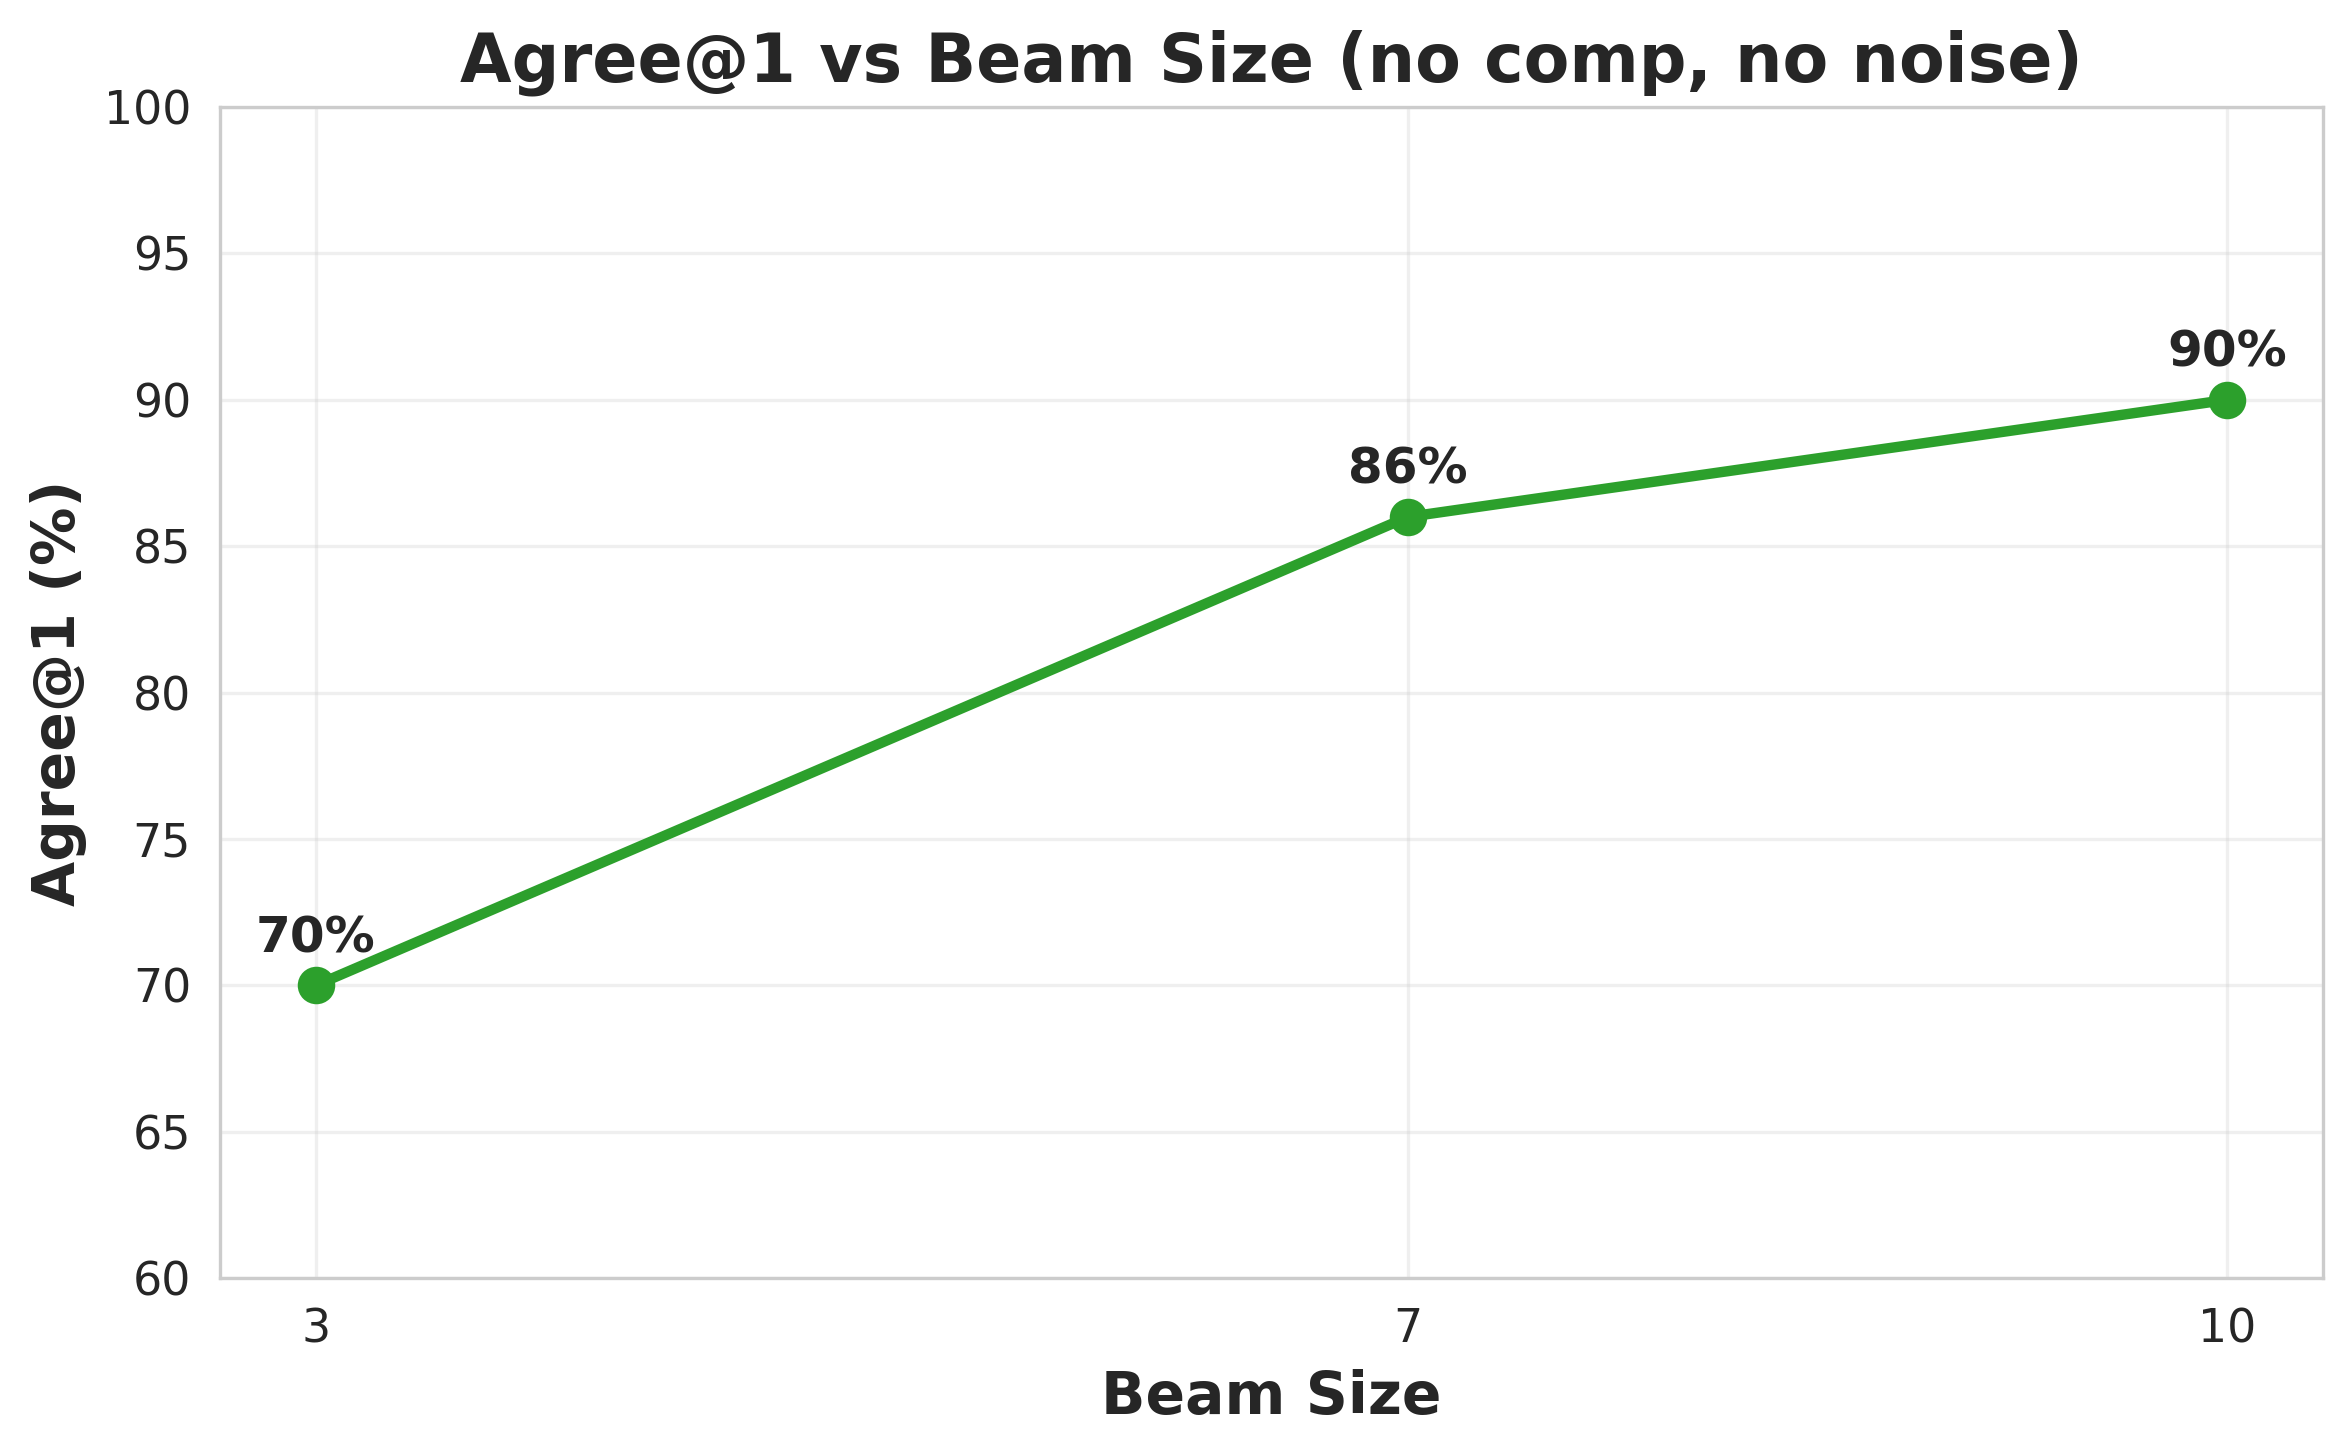
\includegraphics[width=0.45\textwidth]{figures/paper_beam_accuracy.png}
\caption{Top-1 agreement rate increases with beam size under no-compression setting.}
\label{fig:beam_acc}
\end{figure}

\begin{figure}[!t]
\centering
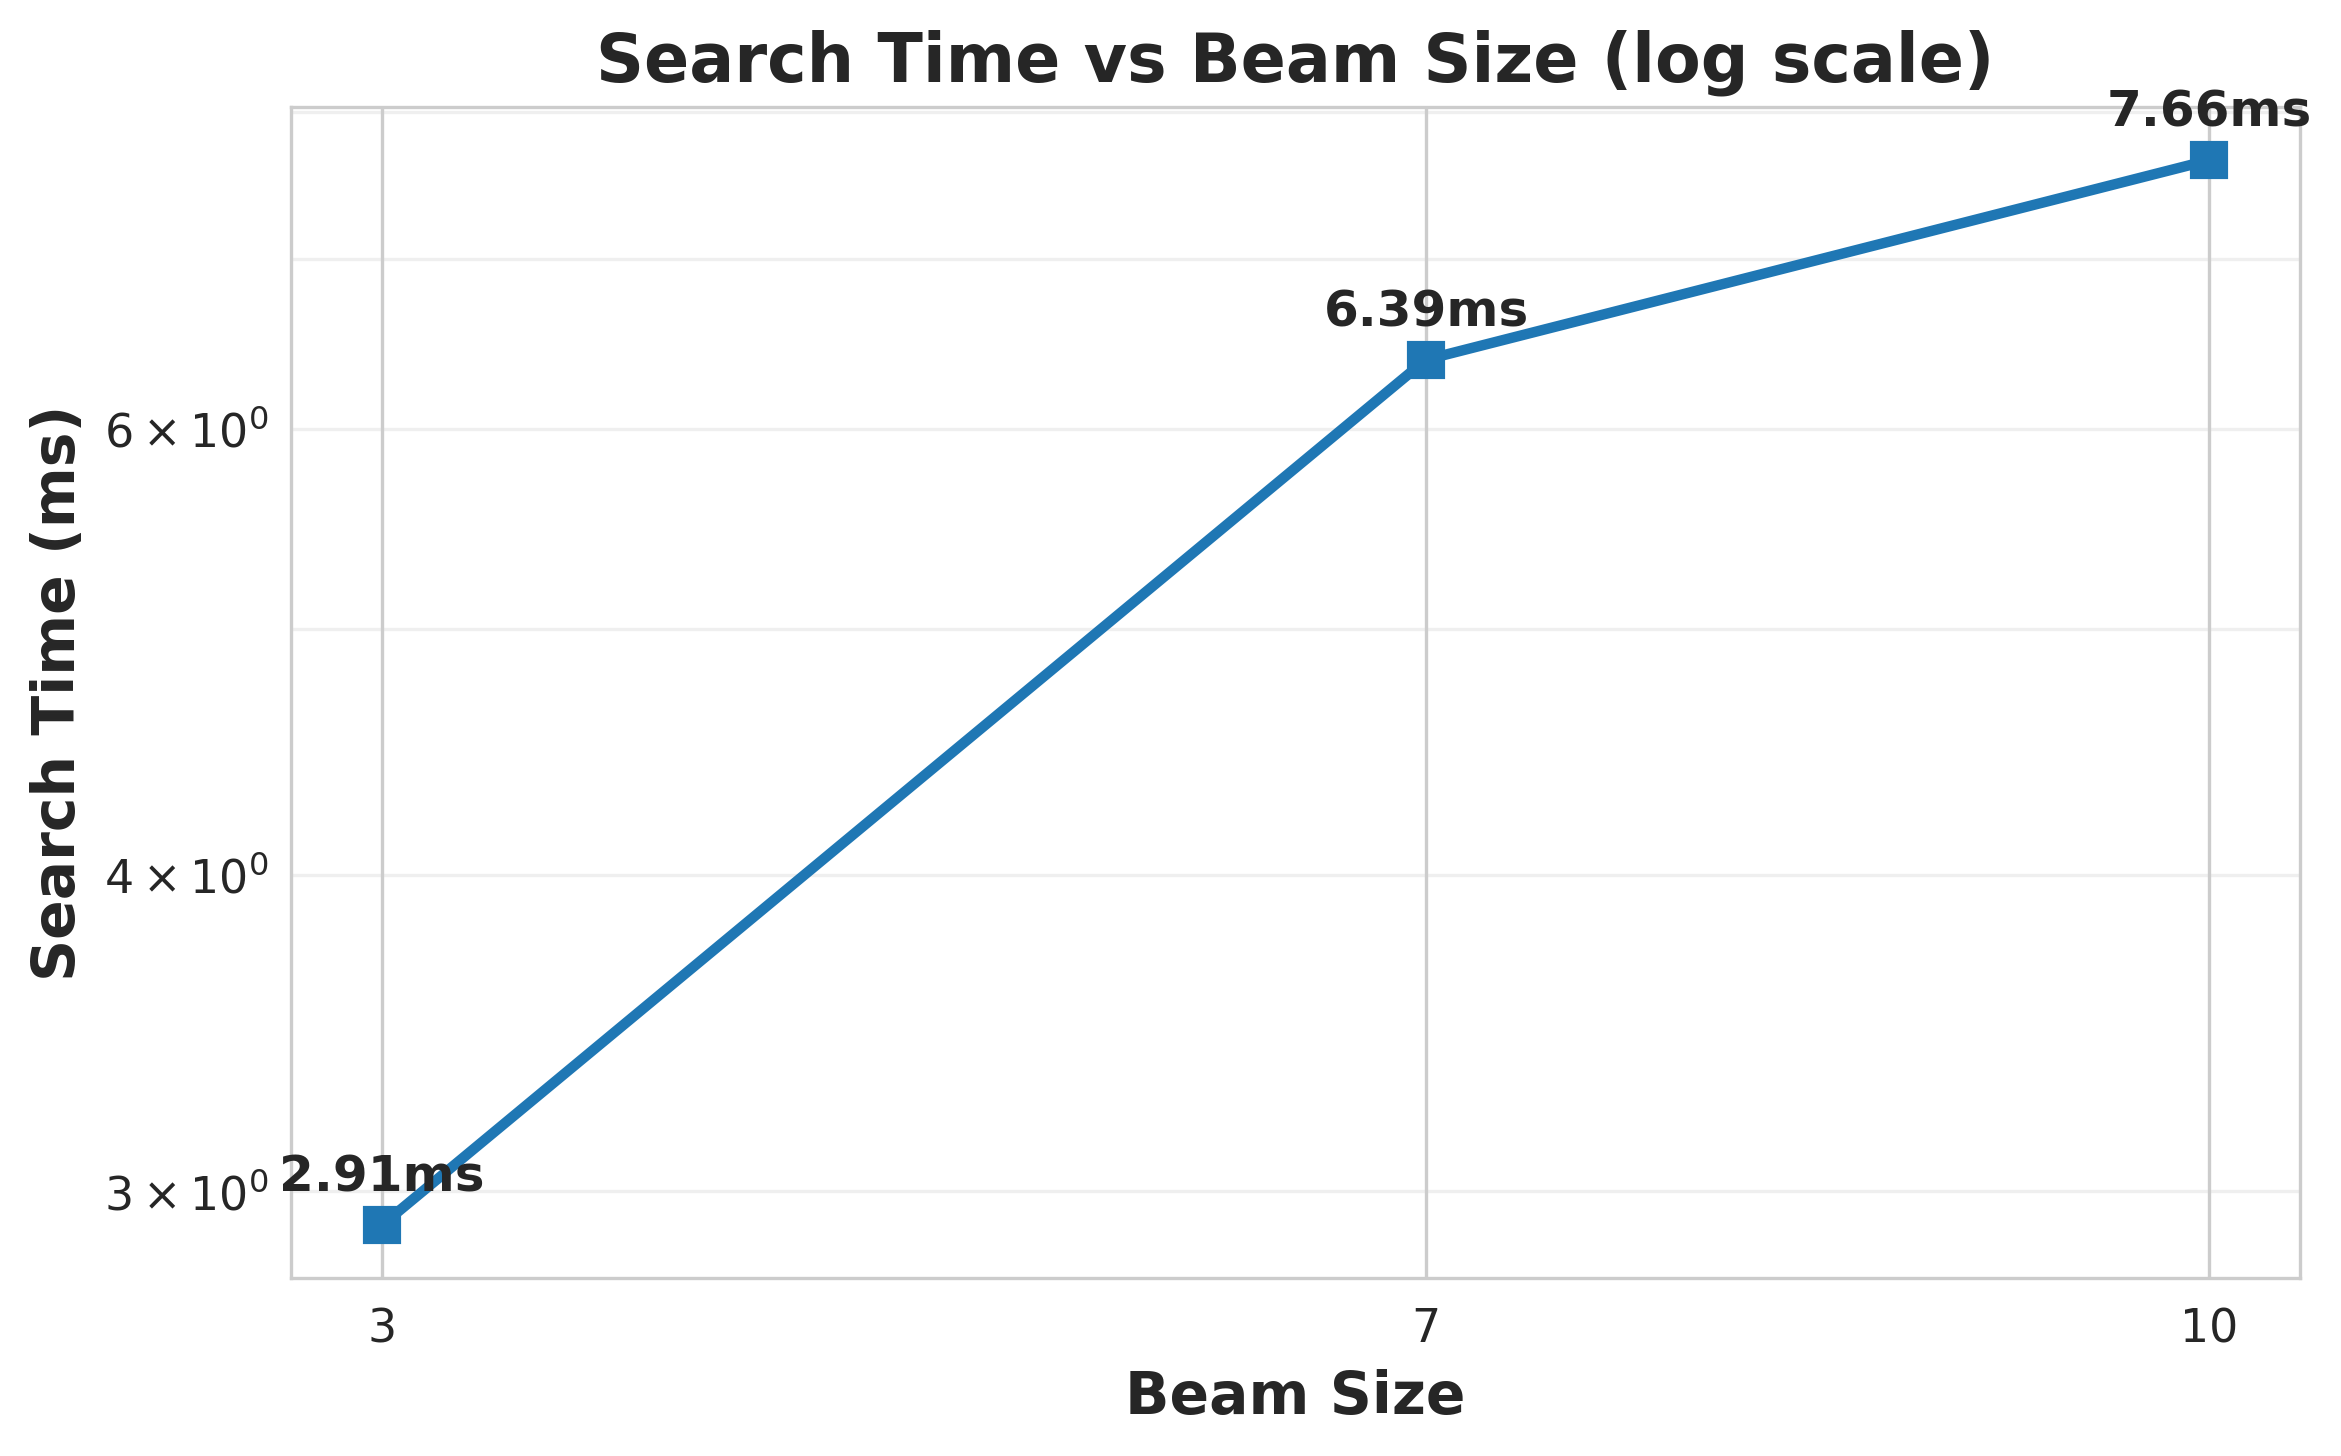
\includegraphics[width=0.45\textwidth]{figures/paper_beam_time.png}
\caption{Search time increases sub-linearly with beam size (log-scale) under no-compression setting.}
\label{fig:beam_time}
\end{figure}

\textbf{Observations}:
\begin{itemize}
    \item \textbf{Diminishing returns}: Increasing beam size improves agreement (e.g., 70\%\,$\to$\,86\%\,$\to$\,90\% for $\beta=3,7,10$), but the marginal gain diminishes at larger beams.
    \item \textbf{Sub-linear time growth}: Search time grows sub-linearly with beam size due to early termination when leaf nodes are reached.
    \item \textbf{Sweet spots}: Beam size 3 for high-throughput scenarios (19.7$\times$ speedup with moderate agreement), and beam size 10 for fidelity-critical scenarios (high agreement, still 7.5$\times$ faster).
\end{itemize}

\subsection{Accuracy--Speed Trade-off}

Fig.~\ref{fig:acc_time_combo} summarizes top-1 agreement (bars, left axis) and average search time (line, right log axis) in one view, highlighting the agreement--efficiency balance achieved by different schemes.

\begin{figure}[!t]
\centering
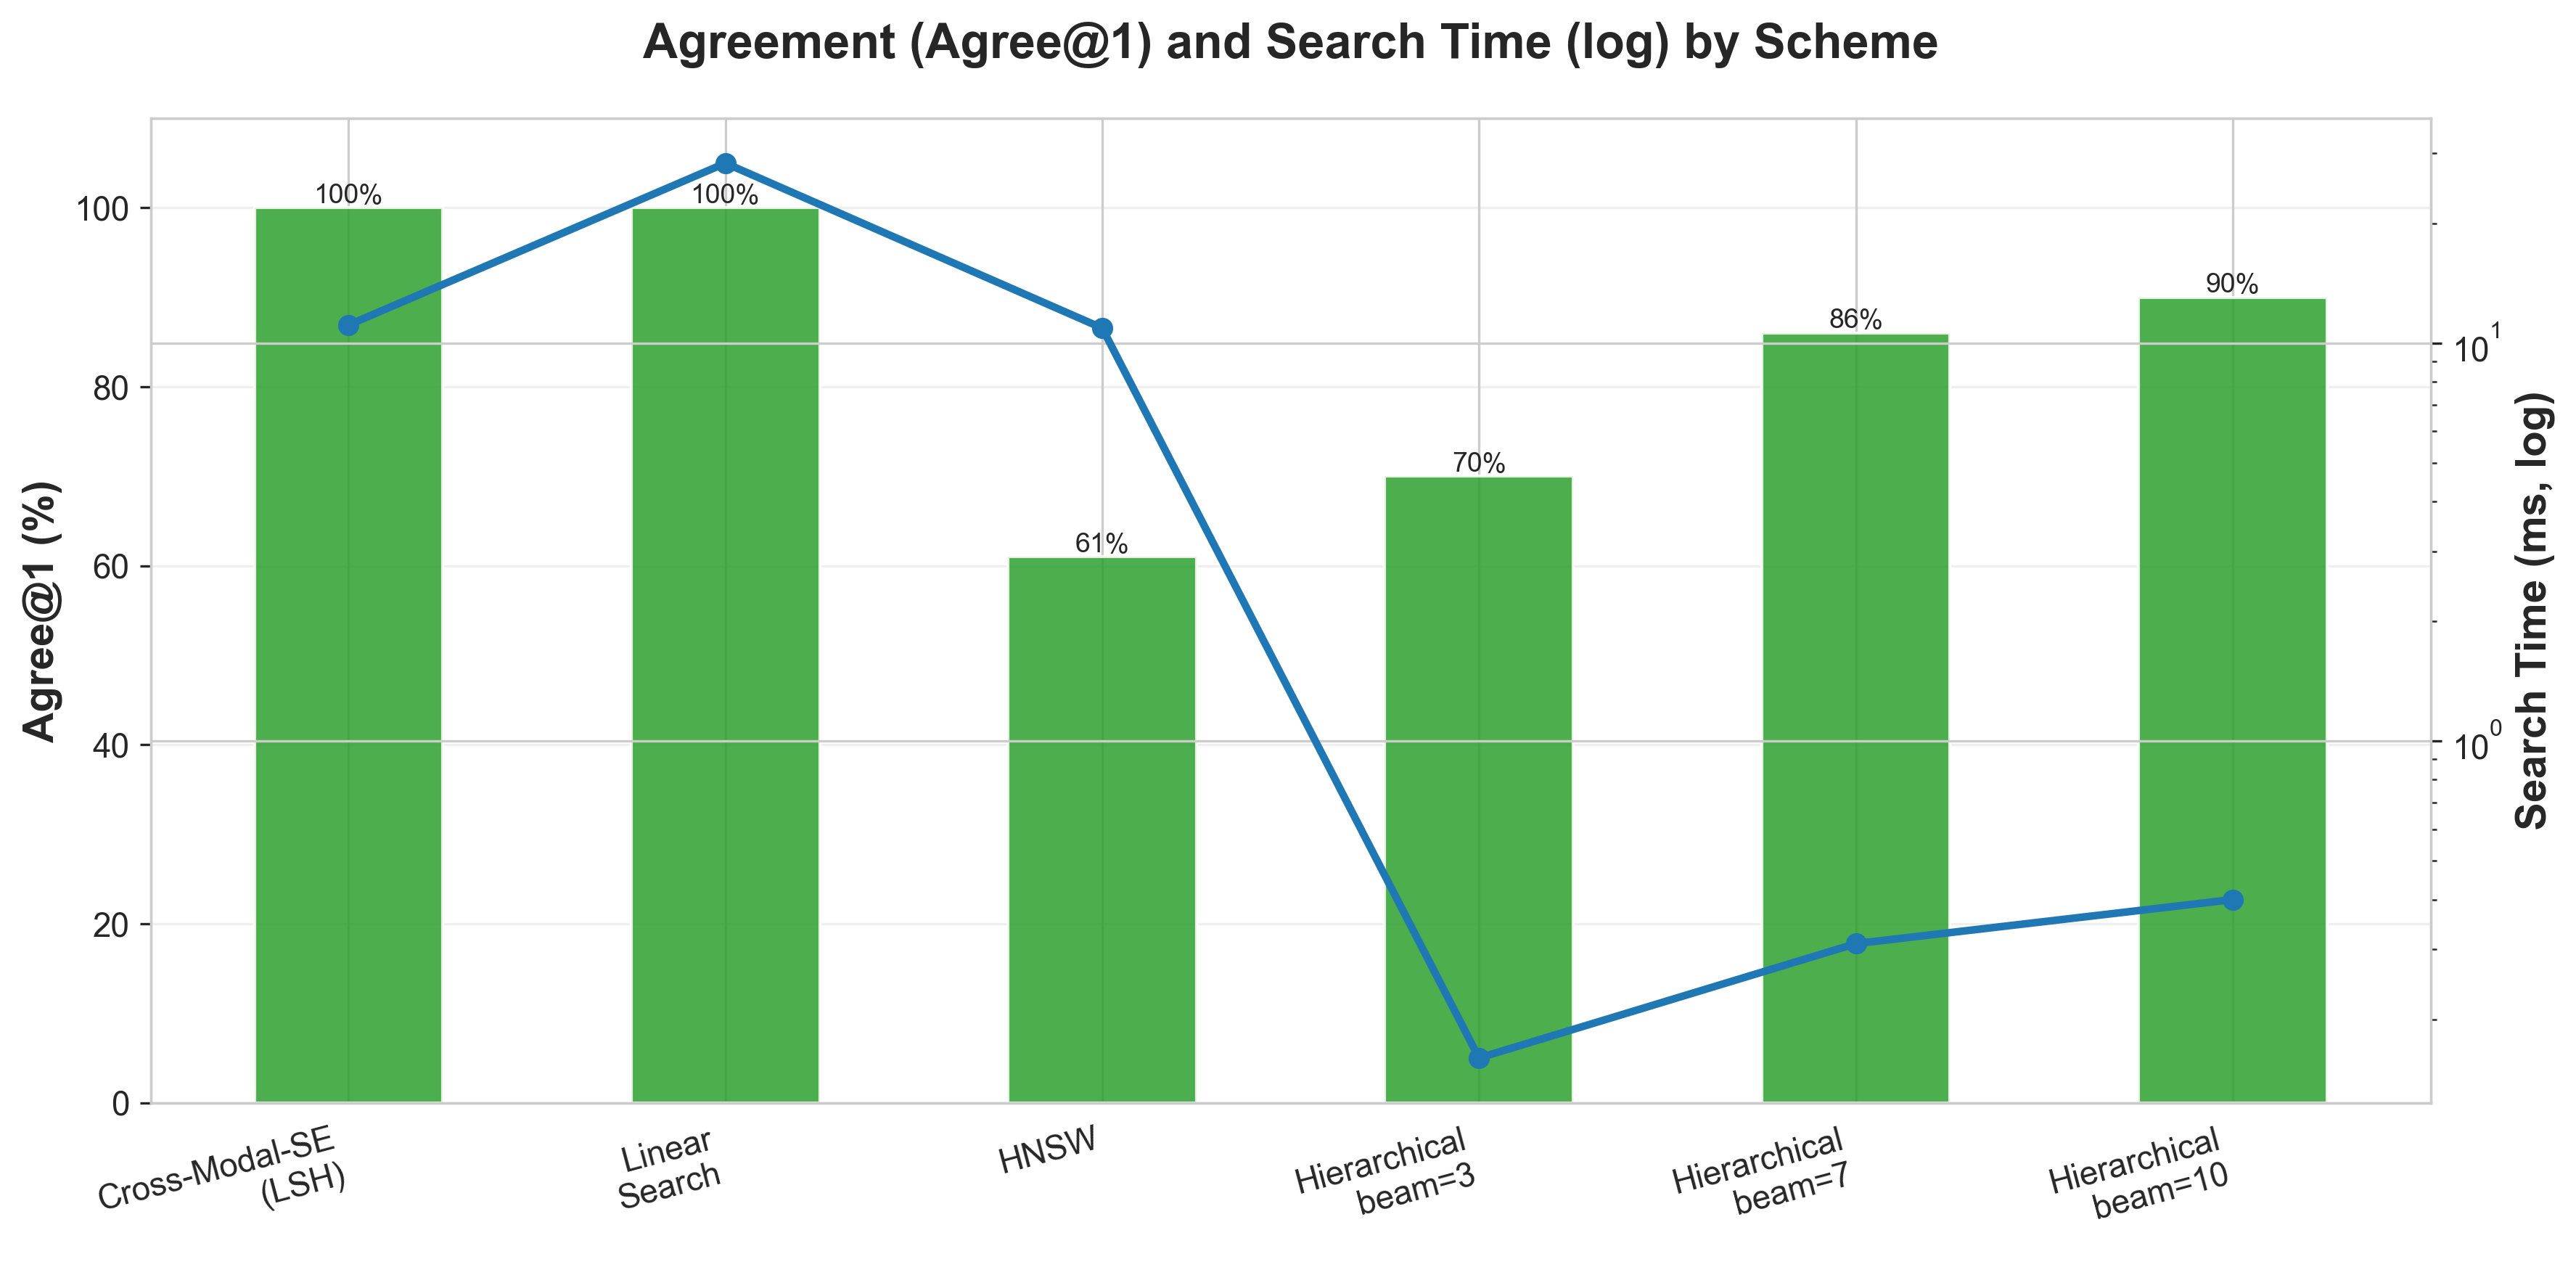
\includegraphics[width=0.48\textwidth]{figures/paper_acc_time_combo.png}
\caption{Agreement-speed trade-off across schemes. Larger beam sizes improve agreement while maintaining millisecond-level latency.}
\label{fig:acc_time_combo}
\end{figure}

\subsection{Noise Robustness (No-Compression Baseline)}

We evaluate robustness under lightweight padding noise on top of the no-compression baseline. Concretely, we add 5\% padding to the vector length ($\ell = 1.05d$) and inject small Gaussian noise ($\sigma=\sigma_q=0.01$) into padding dimensions, leaving original dimensions intact. Our experiments show that (i) lightweight padding noise preserves accuracy—R@1 remains stable within $\pm$2\% across Linear and HST beam sizes; (ii) time overhead is negligible (0--5\%) for HST thanks to sub-linear traversal and fixed tree structure; (iii) separating padding from original dimensions enables security tunability without degrading retrieval quality.


\subsection{Compression Ratio Study and Analysis}
\label{sec:compression_study}

To quantify the impact of dimension reduction alone, we vary the compression ratio $k_\text{ratio}$ under \emph{no noise} and \emph{beam=10} on CIFAR-100. As shown in Fig.~\ref{fig:compression_accuracy}, we observe a striking \emph{non-monotonic} recall pattern: starting from no compression, recall initially \emph{rises} to about 92\% at 2.5\% compression and peaks at about 93\% R@1 with 5\% compression, then declines to 90\% at 7.5\%, 88\% at 10\%, and 86\% at 12.5\% compression. Beyond 10\%, recall continues to degrade (84\% at 15\%, 82\% at 20\%) as informative dimensions are pruned. This counterintuitive improvement at modest compression ratios demonstrates that removing low-variance dimensions can enhance retrieval by reducing noise, though the non-monotonic pattern suggests complex interactions between signal preservation and noise reduction.

\begin{figure}[!t]
\centering
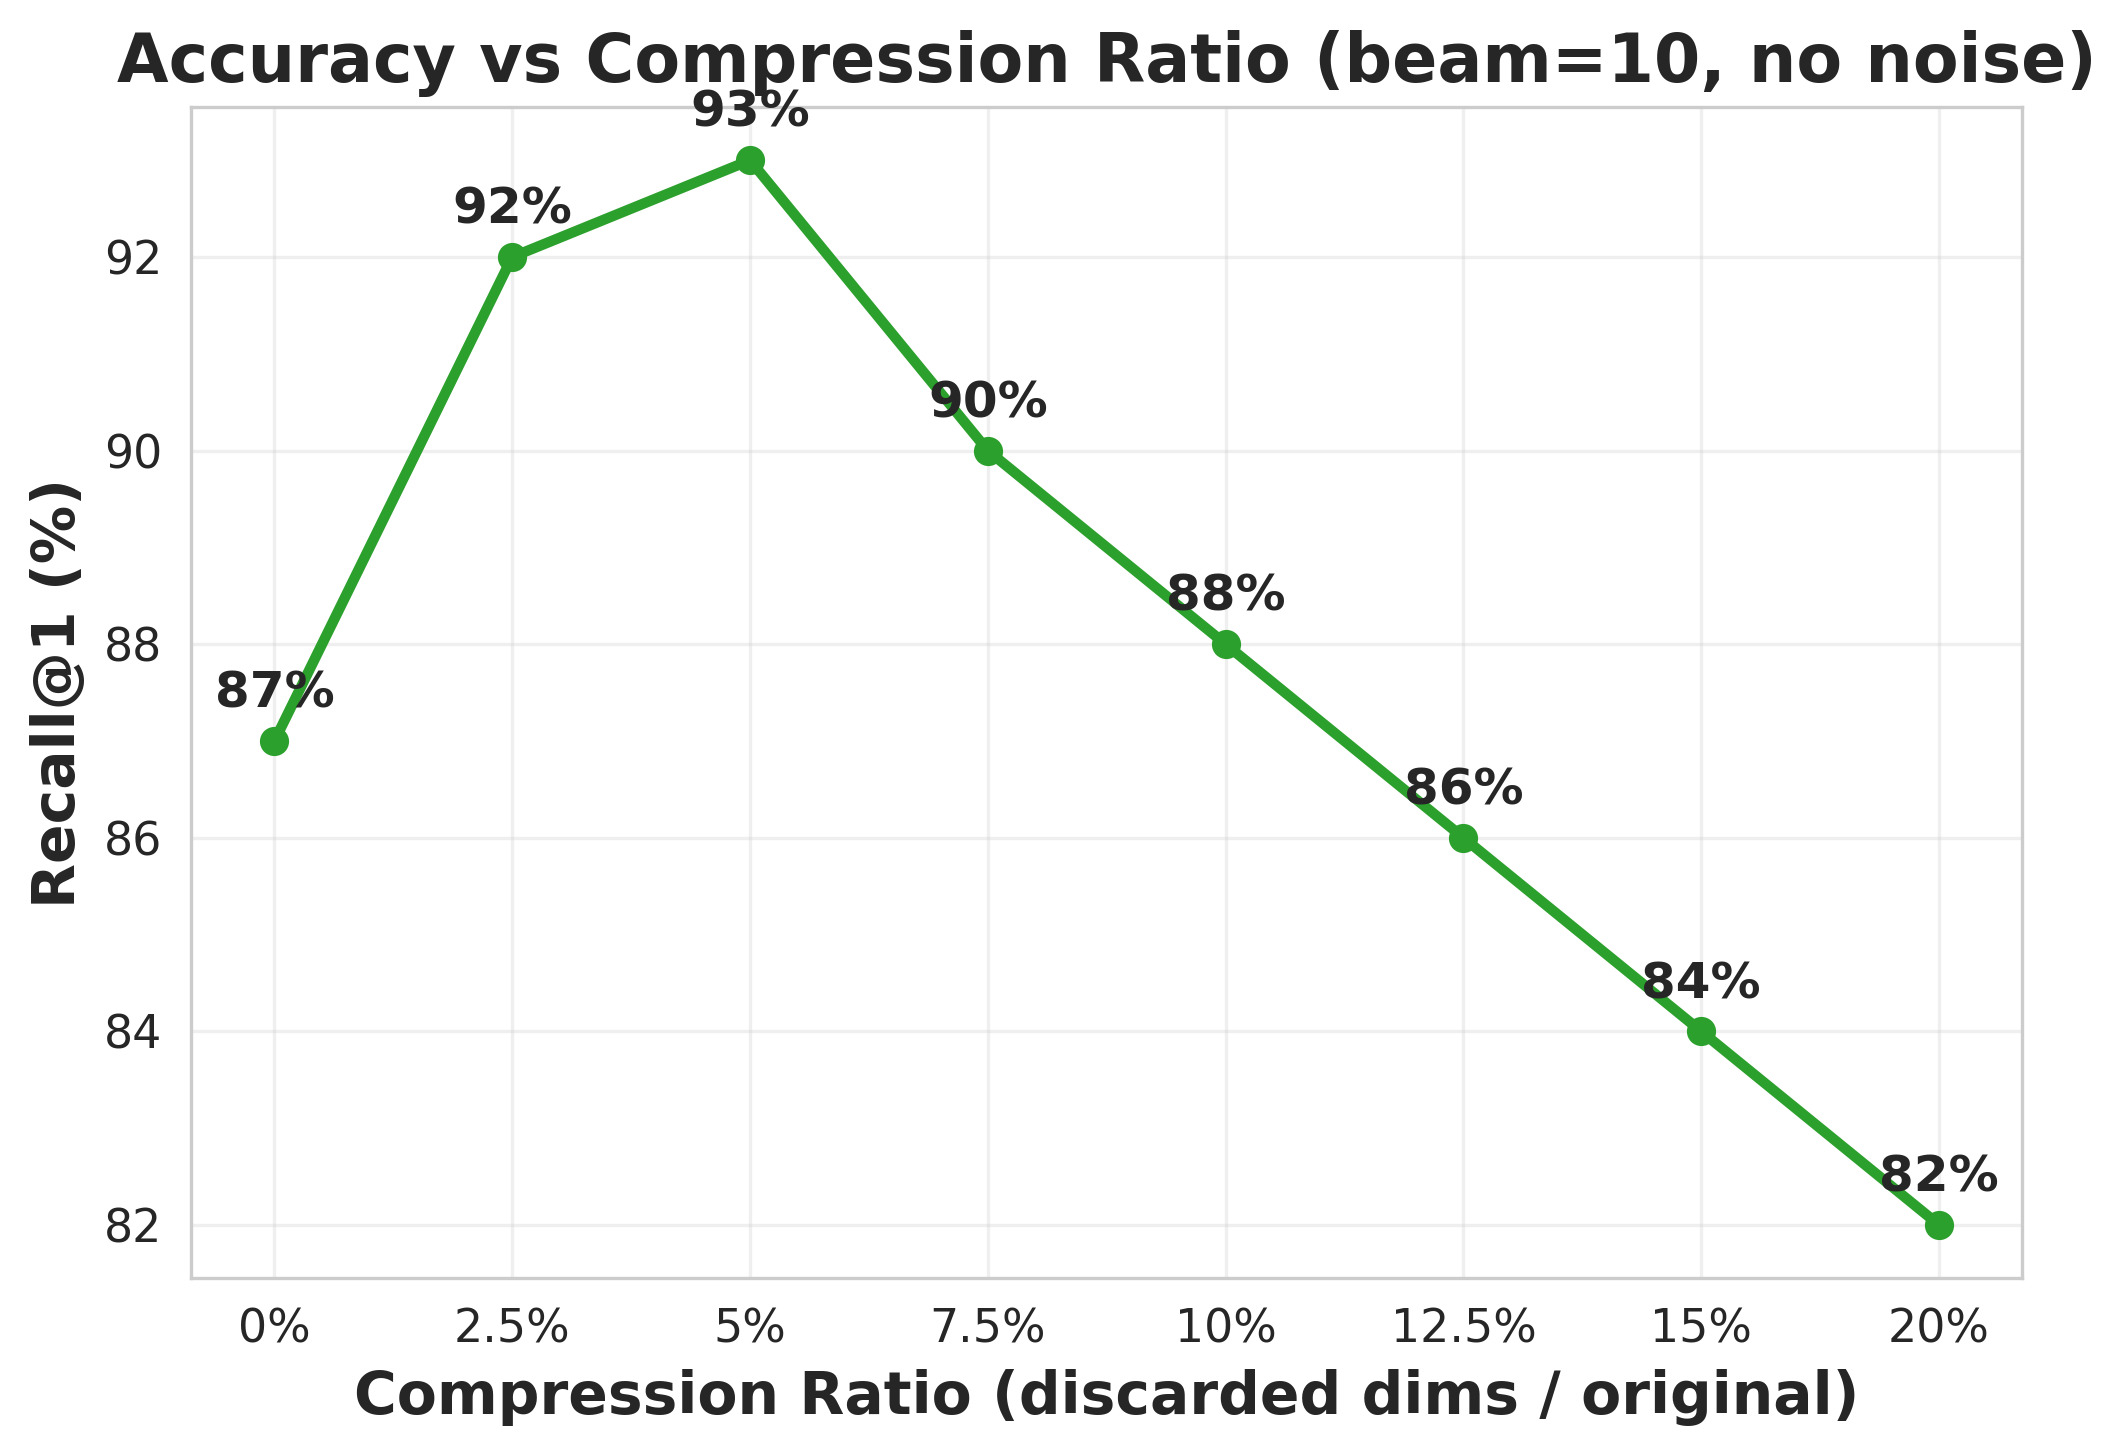
\includegraphics[width=0.48\textwidth]{figures/paper_compression_accuracy.png}
\caption{Non-monotonic relationship between compression ratio and Recall@1 on CIFAR-100. Modest compression (2.5--5\%) improves recall by eliminating low-discriminative dimensions, peaking at 93\% R@1 with 5\% compression. Beyond 10\%, recall degrades as informative dimensions are pruned.}
\label{fig:compression_accuracy}
\end{figure}

\textbf{Theoretical interpretation.}\label{sec:compression_theory}
We explain this trend using a signal-noise decomposition. Let a normalized vector decompose as $\mathbf{d}=\mathbf{s}_d+\boldsymbol{\eta}_d$, where $\mathbf{s}_d$ lies in a signal subspace and $\boldsymbol{\eta}_d$ aggregates weak/irrelevant components. Cosine similarity admits a first-order approximation
\[
\cos(\mathbf{q},\mathbf{d})\;\approx\;\frac{\langle\mathbf{s}_q,\mathbf{s}_d\rangle+\langle\boldsymbol{\eta}_q,\boldsymbol{\eta}_d\rangle}{\sqrt{(\|\mathbf{s}_q\|^2+\|\boldsymbol{\eta}_q\|^2)(\|\mathbf{s}_d\|^2+\|\boldsymbol{\eta}_d\|^2)}}.
\]
Removing weak-variance coordinates reduces the denominator and the variance of spurious terms $\langle\boldsymbol{\eta}_q,\boldsymbol{\eta}_d\rangle$, improving the separation between true and distractor similarities. On the hierarchical spherical tree, this decreases center-angle jitter and the probability of branching mistakes in beam search. When compression exceeds a threshold and starts pruning informative coordinates, the numerator $\langle\mathbf{s}_q,\mathbf{s}_d\rangle$ diminishes and recall degrades. This explains the observed ``initial rise then fall'' without contradicting the information-loss intuition.

\subsection{Index Construction Time}

Table~\ref{tab:index_construction} compares index construction time and memory overhead on the full CIFAR-100 dataset (50{,}000 images).

\begin{table}[!t]
\centering
\caption{Index Construction Metrics on CIFAR-100 (50{,}000 images)}
\label{tab:index_construction}
\begin{tabular}{lcc}
\toprule
\textbf{Scheme} & \textbf{Construction Time} (s) & \textbf{Index Size} (MB) \\
\midrule
Cross-Model-SE & 10.27 & 518.89 \\
PITR & 11.50 & 28.5 \\
Linear Search & 7.73 & 782.10 \\
VCSE-HST & 10.08 & 782.10 \\
\bottomrule
\end{tabular}
\end{table}

VCSE-HST's index construction time (10.08s) is comparable to Cross-Model-SE (10.27s) and faster than PITR (11.50s), while being slightly higher than Linear Search (7.73s) due to the additional overhead of hierarchical tree construction and Merkle commitment computation. PITR's longer construction time reflects the cost of building HNSW's multi-layer graph structure. The index size is larger than Cross-Model-SE (782MB vs 519MB) because we store full encrypted vectors rather than compact hash codes, though still significantly larger than PITR's compressed representation (28.5MB). However, the memory overhead is acceptable for modern systems, and the significant search speedup (7.5--19.7$\times$ over Cross-Model-SE) justifies this trade-off.

\subsection{Integrity Verification Overhead}

We evaluate the cost of Merkle-tree-based integrity verification on CIFAR-100 using our reports with $\beta\in\{1,3,5,7,10\}$. Fig.~\ref{fig:merkle_time_vs_beam} shows that average per-query verification time scales near-linearly with beam size and remains in the few-millisecond range. Fig.~\ref{fig:merkle_breakdown} decomposes total latency into search and verification components.

\begin{figure}[!t]
\centering
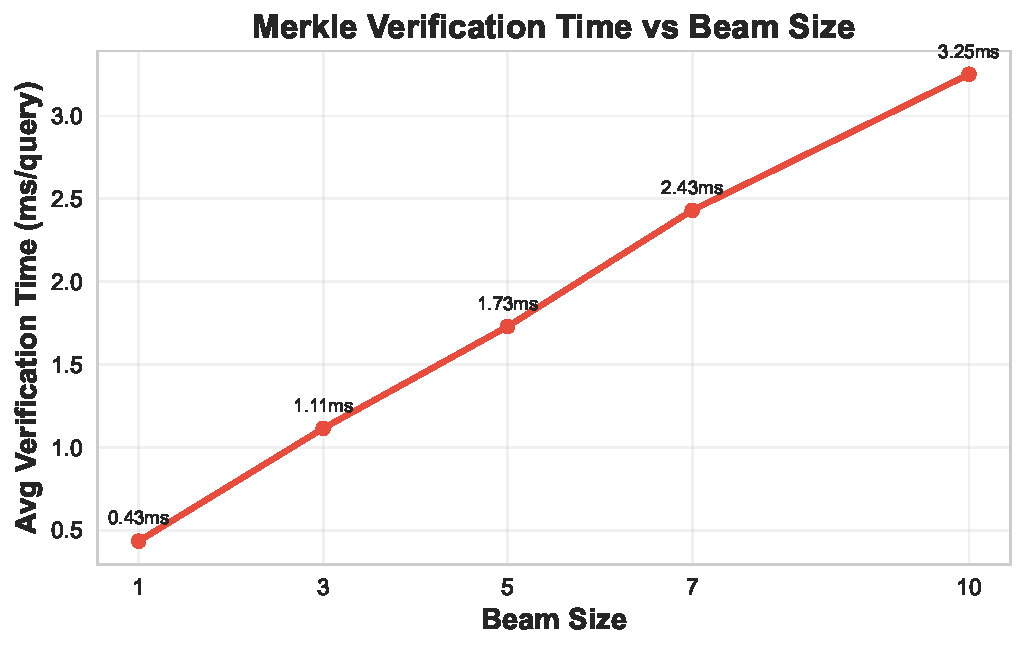
\includegraphics[width=0.48\textwidth]{figures/paper_merkle_verification_time_vs_beam.pdf}
\caption{Verification time vs beam size for Merkle-based integrity checks. Overhead grows near-linearly with $\beta$ and stays within a few milliseconds per query.}
\label{fig:merkle_time_vs_beam}
\end{figure}

\begin{figure}[!t]
\centering
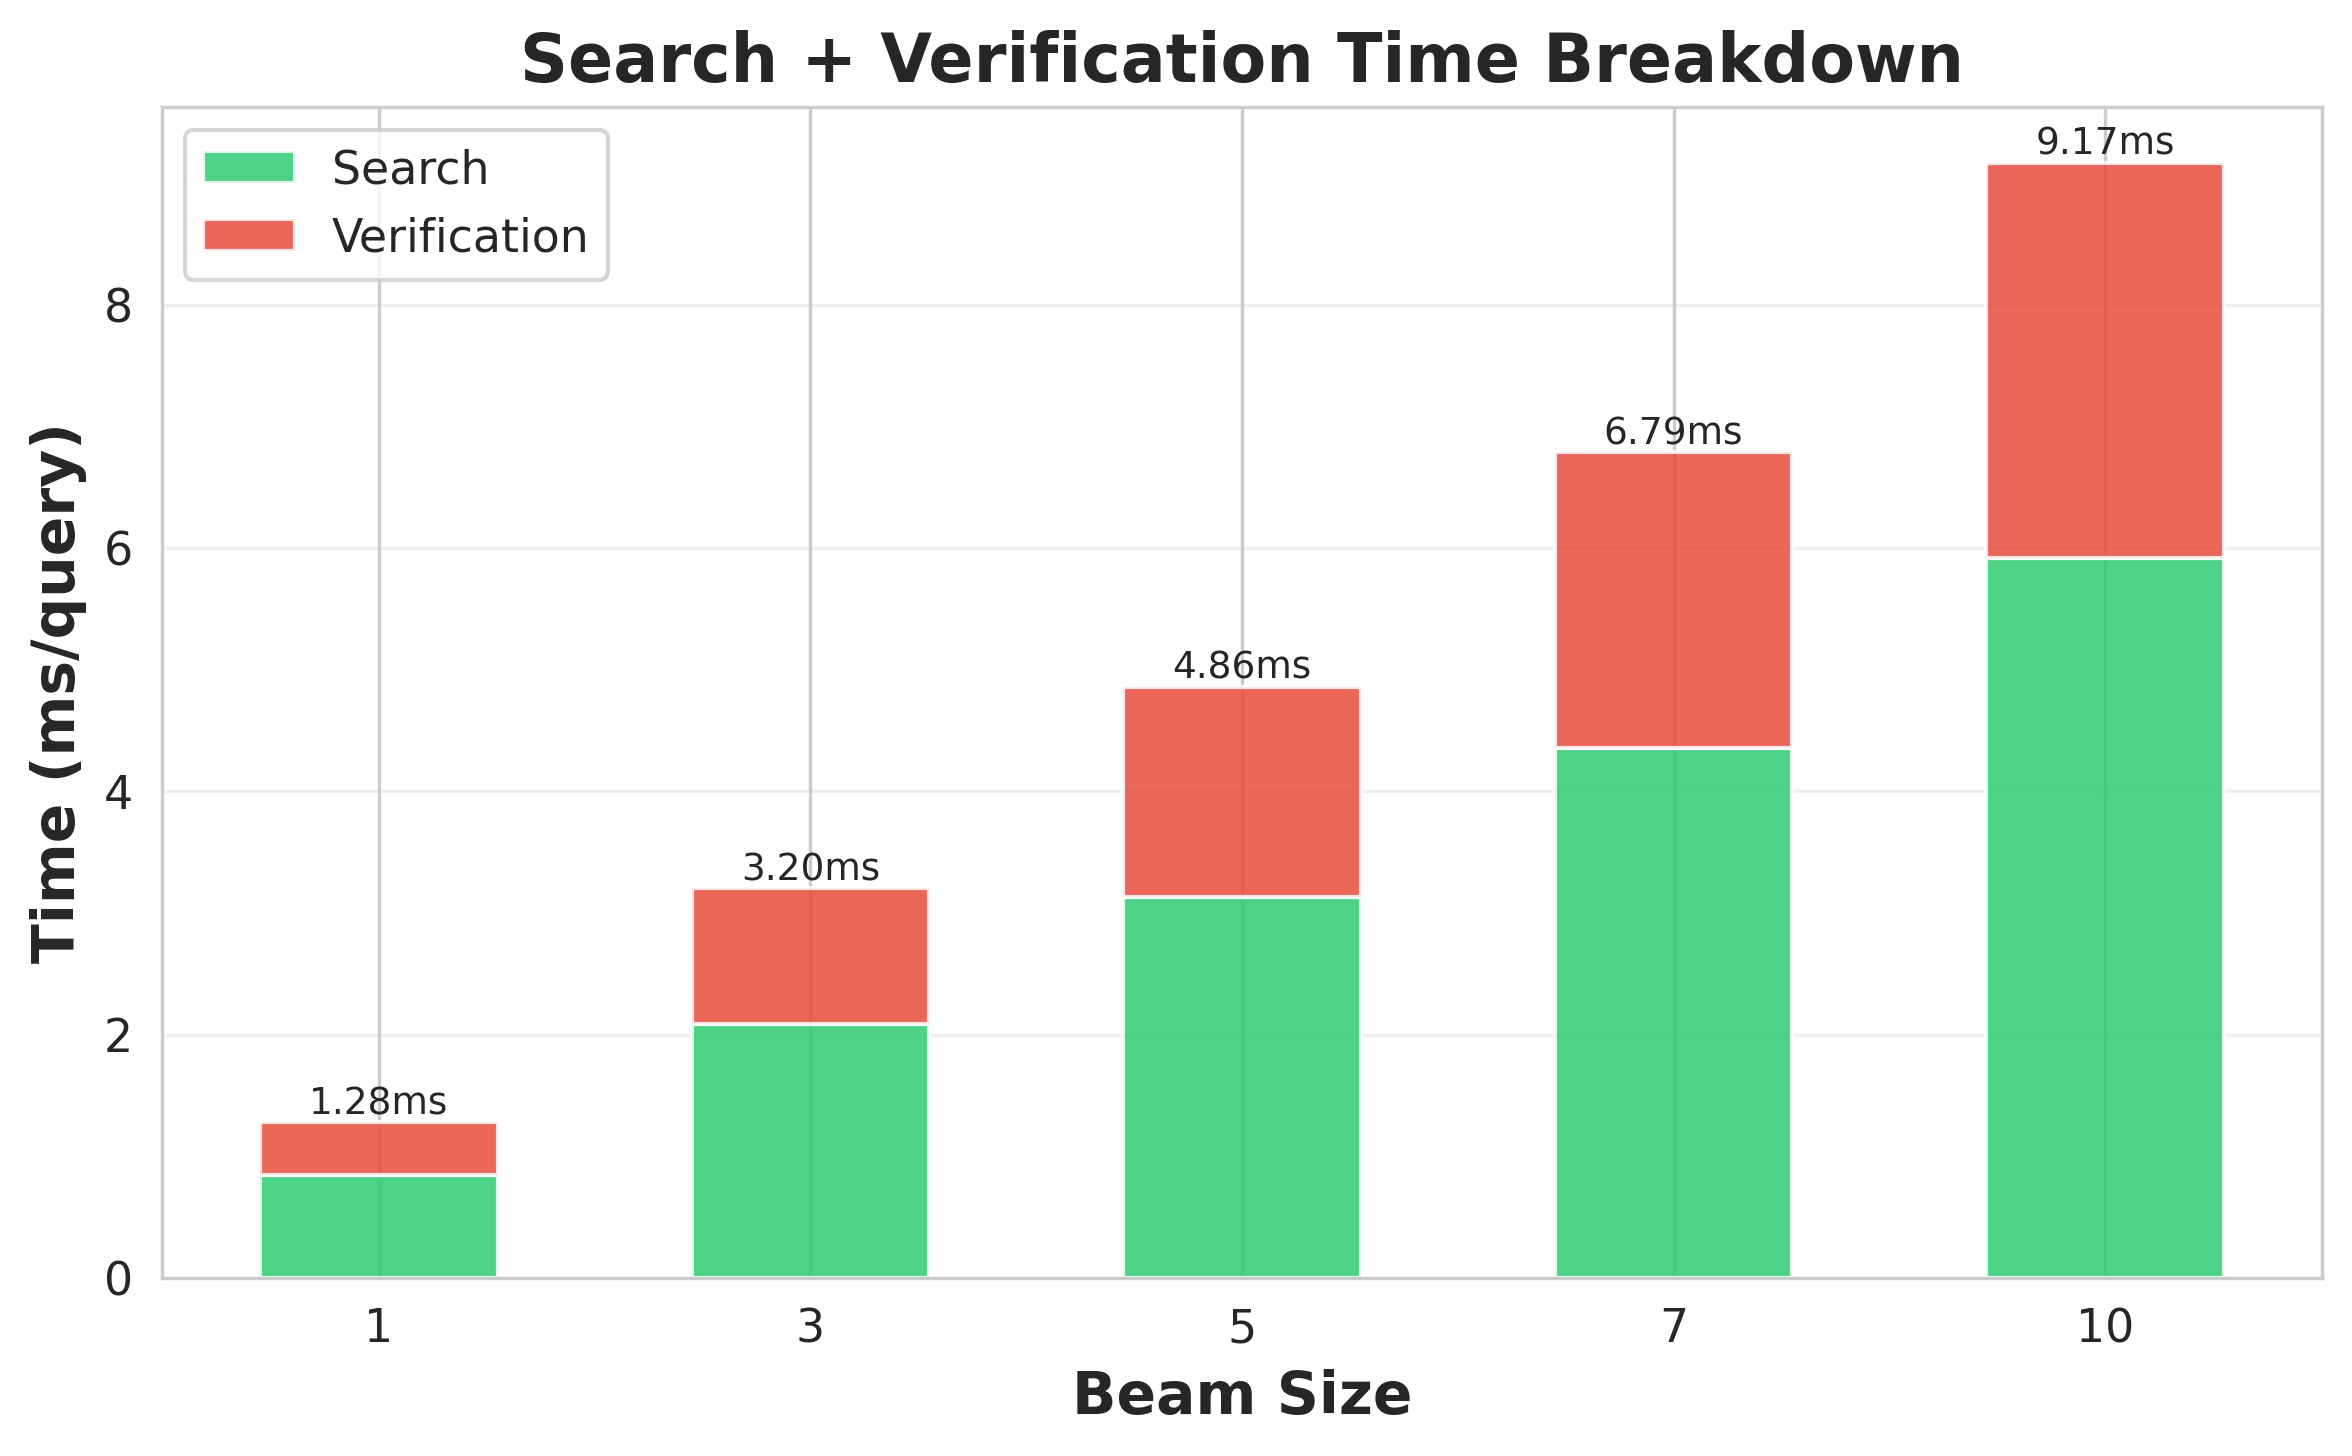
\includegraphics[width=0.48\textwidth]{figures/paper_merkle_time_breakdown.png}
\caption{Per-query latency breakdown (search + verification). Verification constitutes a small fraction of total time and does not change accuracy metrics.}
\label{fig:merkle_breakdown}
\end{figure}

Finally, Fig.~\ref{fig:merkle_index_time} summarizes the average index construction overhead introduced by adding Merkle commitments; the extra hashing is modest compared to overall preprocessing.

\begin{figure}[!t]
\centering
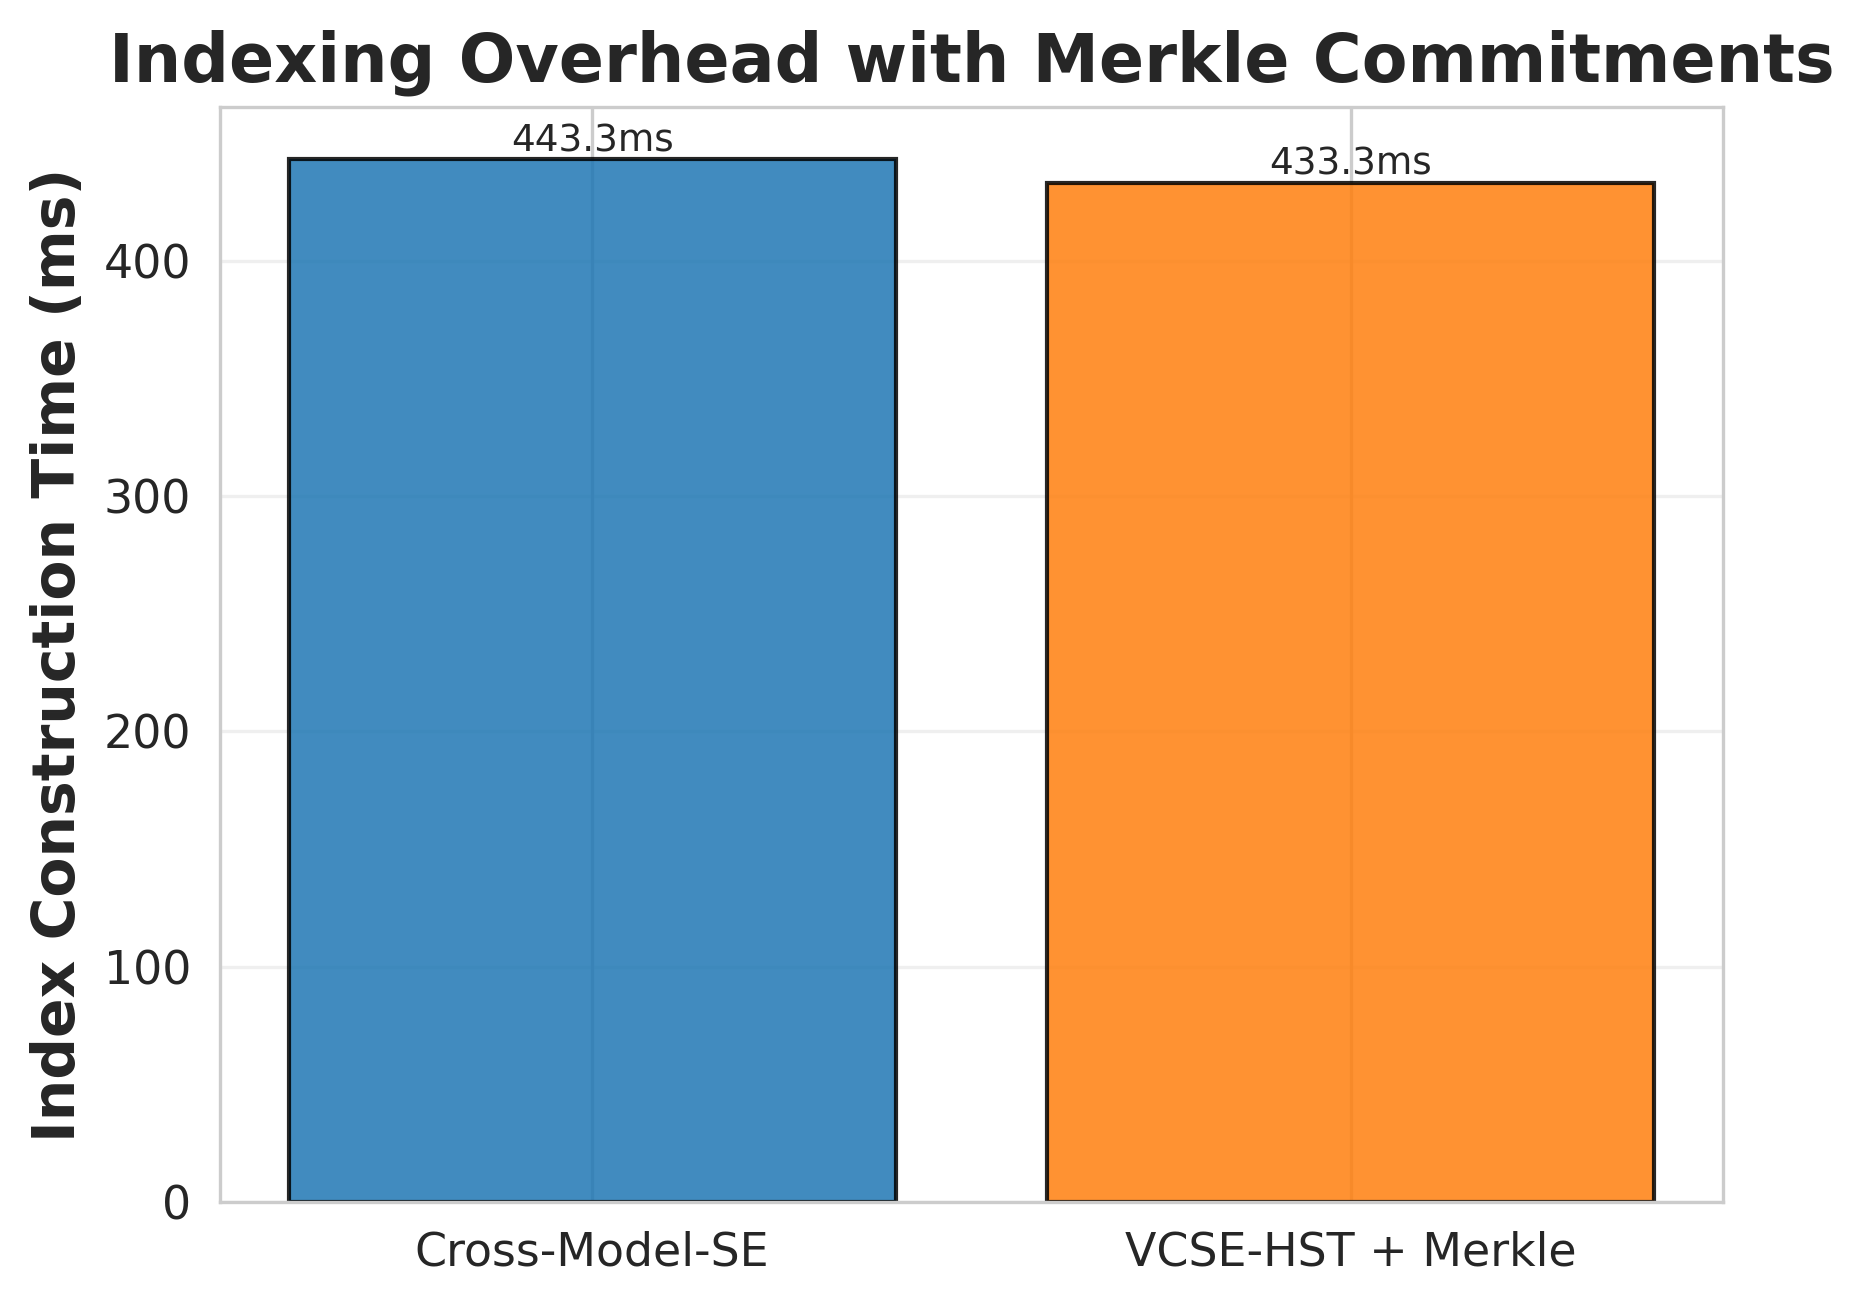
\includegraphics[width=0.45\textwidth]{figures/paper_merkle_index_time.png}
\caption{Index construction time: Cross-Model-SE vs VCSE-HST + Merkle (ms). Merkle hashing adds modest overhead at build time.}
\label{fig:merkle_index_time}
\end{figure}

\textbf{Limitation}. The Merkle layer guarantees execution integrity \emph{with respect to the chosen beam size $\beta$} (path completeness and result inclusion along the executed search). It does not guarantee global top-$k$ completeness beyond the beam-search exploration. The verification cost grows approximately linearly with $\beta$.

% (Scalability discussion removed per revision focus.)
\section{Conclusion}
\label{sec:conclusion}

In this paper, we proposed VCSE-HST, a verifiable cross-modal searchable encryption scheme based on a hierarchical spherical tree with beam search. By constructing a shallow $k$-ary tree and employing beam search to avoid local optima, our scheme attains strong accuracy–efficiency trade-offs: on CIFAR-100 (50{,}000) and Caltech256 (30{,}607), beam size 10 matches Cross-Model-SE (90\% R@1) while being 7.5$\times$ faster; beam size 3 yields up to 19.7$\times$ speedup with ~7\% R@1 drop.

We enable \emph{score-consistency verification} under encryption: clients check the correctness of returned scores using lightweight auxiliary coefficients, and we enforce \emph{execution integrity} of beam search via Merkle commitments. We do not claim global optimality beyond the beam-search approximation. Security analysis shows that VCSE-HST protects index, query, and keyword privacy under honest-but-curious adversaries.

\noindent\textbf{Limitation.} Our scheme does not hide access/search patterns: the server can observe returned identifiers and the set of visited nodes. Beam search explores multiple paths and may reveal a larger visited-node set than greedy search; protecting patterns requires orthogonal techniques (e.g., ORAM, DPF), which we leave to future work.

Future work includes: (1) extending the scheme to support dynamic updates with forward and backward security, (2) exploring adaptive beam size strategies based on query characteristics, (3) optimizing index compression to reduce memory overhead, and (4) evaluating scalability on larger datasets (e.g., 100K+ documents). We also plan to investigate hybrid index structures combining hierarchical trees with locality-sensitive hashing for even better performance on ultra-large-scale datasets.

\section*{Acknowledgment}

The author would like to thank the anonymous reviewers for their valuable comments and suggestions.

\bibliographystyle{IEEEtran}
\bibliography{references}

\vspace{12pt}

\end{document}
